% !TeX program = xetex
\documentclass[xcolor={table,usenames,dvipsnames}]{beamer}
\usepackage{eso-pic} 
\usepackage[absolute,overlay]{textpos}
\usepackage{colortbl}
\usepackage{fourier}
\usepackage{booktabs}% http://ctan.org/pkg/booktabs
\newcommand{\tabitem}{~~\llap{\textbullet}~~}
\usepackage{tabularx}
\usepackage{tikz}
\usetikzlibrary{positioning}
\usetikzlibrary{arrows.meta}

\setbeamertemplate{blocks}[rounded][shadow=true]
\let\olditem\item
\renewcommand{\item}{%
\olditem\vspace{0pt}}     
\usepackage{ragged2e}


%\usepackage[round]{natbib} % incompatible avec biblatex
\usepackage{hyperref}
\hypersetup{
    colorlinks=true,
    linkcolor=.,
    filecolor=deepblue,      
    urlcolor=deepblue,
    pdftitle={Overleaf Example},
    pdfpagemode=FullScreen,
    citecolor=deepblue
    }
\definecolor{LightCyan}{rgb}{0.88,1,1}   
\usepackage[justification=centering]{caption}
\captionsetup{font=scriptsize}
\captionsetup[figure]{name=Fig.}
\captionsetup[table]{name=Tab.}
\setbeamertemplate{caption}[numbered]
\usepackage[T1]{fontenc}
\usepackage{ctex}
\UseRawInputEncoding
%\usepackage[backend=bibtex, style=authoryear, natbib=true, sorting=nty, backref=true]{biblatex}
%%%% TOUCHE PLUS LE STYLE DE CITATION !!
\usepackage[style=authoryear, maxbibnames=99, mincitenames=1, maxcitenames=2, backref=true, hyperref=true, dashed=false, firstinits=true, backend=bibtex, bibencoding=utf8, uniquename=false, uniquelist=false, natbib=true]{biblatex}
\renewcommand*{\bibfont}{\footnotesize}
\setbeamerfont{footnote}{size=\tiny}

% Remove quotation marks from titles
\DeclareFieldFormat[article,incollection,inproceedings,conference]{title}{#1} 
\addbibresource{bibliographie.bib}

%\usepackage[backend=bibtex,
%style=authoryear,
%natbib=true,
%sorting=nty,
%backref=true
%]{biblatex}

\let\oldnocite\nocite
\makeatletter
\renewcommand*{\nocite}[1]{\oldnocite{#1}\Hy@backout{#1}}
\makeatother

\renewcommand*{\bibfont}{\footnotesize}

\DeclareCiteCommand{\cite}
  {\usebibmacro{prenote}}
  {\usebibmacro{citeindex}%
   \printtext[bibhyperref]{\usebibmacro{cite}}}
  {\multicitedelim}
  {\usebibmacro{postnote}}

\DeclareCiteCommand*{\cite}
  {\usebibmacro{prenote}}
  {\usebibmacro{citeindex}%
   \printtext[bibhyperref]{\usebibmacro{citeyear}}}
  {\multicitedelim}
  {\usebibmacro{postnote}}

\DeclareCiteCommand{\parencite}[\mkbibparens]
  {\usebibmacro{prenote}}
  {\usebibmacro{citeindex}%
    \printtext[bibhyperref]{\usebibmacro{cite}}}
  {\multicitedelim}
  {\usebibmacro{postnote}}

\DeclareCiteCommand*{\parencite}[\mkbibparens]
  {\usebibmacro{prenote}}
  {\usebibmacro{citeindex}%
    \printtext[bibhyperref]{\usebibmacro{citeyear}}}
  {\multicitedelim}
  {\usebibmacro{postnote}}

\DeclareCiteCommand{\footcite}[\mkbibfootnote]
  {\usebibmacro{prenote}}
  {\usebibmacro{citeindex}%
  \printtext[bibhyperref]{ \usebibmacro{cite}}}
  {\multicitedelim}
  {\usebibmacro{postnote}}

\DeclareCiteCommand{\footcitetext}[\mkbibfootnotetext]
  {\usebibmacro{prenote}}
  {\usebibmacro{citeindex}%
   \printtext[bibhyperref]{\usebibmacro{cite}}}
  {\multicitedelim}
  {\usebibmacro{postnote}}

%\DeclareCiteCommand{\textcite}
%  {\boolfalse{cbx:parens}}
%  {\usebibmacro{citeindex}%
%   \printtext[bibhyperref]{\usebibmacro{textcite}}}
%  {\ifbool{cbx:parens}
%     {\bibcloseparen\global\boolfalse{cbx:parens}}
%     {}%
%   \multicitedelim}
%  {\usebibmacro{textcite:postnote}}

        \DeclareCiteCommand{\textcite}
        {\usebibmacro{cite:init}%
            \usebibmacro{prenote}}
        {\usebibmacro{citeindex}%
            \printtext[bibhyperref]{\usebibmacro{textcite}}}
        {}
        {\printtext[bibhyperref]{\usebibmacro{textcite:postnote}}%
            \usebibmacro{cite:post}}

%\addbibresource{bibliographie.bib}

% Cannot enable in Xelatex
\usepackage{pgfpages}
% \setbeameroption{hide notes} % Only slides
% \setbeameroption{show only notes} % Only notes
% \setbeameroption{show notes on second screen}

% other packages
\usepackage{latexsym,amsmath,multicol,booktabs,calligra}
\usepackage{graphicx,listings,stackengine}
\usepackage[greek,french]{babel}
\usepackage[LGR,T1]{fontenc}
\usepackage{fontspec}

%\usepackage[sfdefault,light,led=.85]{merriweather} %% Option 'black' gives heavier bold face 


\usepackage[sfdefault]{AlegreyaSans} %% Option 'black' gives heavier bold face
%% The 'sfdefault' option to make the base font sans serif
\renewcommand*\oldstylenums[1]{{\AlegreyaSansOsF #1}}



% Define a command for text in Greek. Replace 'Gentium Plus' with a font of your choice if necessary.
%\newfontfamily\greekfont{Gentium Plus}
%\newcommand{\textgreek}[1]{{\greekfont #1}}

\DefineBibliographyStrings{french}{%
  backrefpage = {voir p\adddot},%
  backrefpages = {voir pp\adddot}%
}
\DeclareFieldFormat{pagerefformat}{\mkbibparens{{\color{red}\mkbibemph{#1}}}}
\renewbibmacro*{pageref}{%
  \iflistundef{pageref}
    {}
    {\printtext[pagerefformat]{%
       \ifnumgreater{\value{pageref}}{1}
         {\bibstring{backrefpages}\ppspace}
         {\bibstring{backrefpage}\ppspace}%
       \printlist[pageref][-\value{listtotal}]{pageref}}}}
\usepackage{wasysym}
% Enable only in Xelatex
 \usepackage{pstricks}

\author[Ljudmila PETKOVIC]{\small \textbf{Ljudmila PETKOVIC}\textsuperscript{1,2,3,4}\\\medskip{\footnotesize\texttt{prenom.nom@sorbonne-universite.fr}}}
\title[Extraction terminologique $\cdot$ circulation des savoirs $\cdot$ corpus Charcot]{\fontsize{13pt}{16pt}\selectfont L'extraction terminologique : un levier pour analyser la circulation des savoirs ? Le cas du corpus Charcot.}
%\subtitle{Approche \textit{PatternRank}}
\institute [JE \og{}Humanités numériques\fg{}] {\tiny \textsuperscript{1} Sorbonne Université, Faculté des Lettres, \textsc{UFR} Littératures françaises et comparée, \textsc{ED III} (\textsc{ED019})\\\textsuperscript{2} Sorbonne Université, Centre d'étude de la langue et des littératures françaises (\textsc{CELLF}), \textsc{UMR 8599}\\\textsuperscript{3} Sorbonne Université, Observatoire des textes, des idées et des corpus (\textsc{ObTIC})\\\textsuperscript{4} Sorbonne Université, \textsc{UFR} Sociologie et Informatique pour les Sciences Humaines}
\date[Journée de travail \textsc{ARIANE} (\textsc{GT4}), 17/06/2025]{\scriptsize Journée de travail du consortium \textsc{ARIANE} (\textsc{GT4}) \\\textsc{SCAI}, salle du Conseil\\Paris, le 17 juin 2025}
\usepackage{YTU}

% defs
\def\cmd#1{\texttt{\color{red}\footnotesize $\backslash$#1}}
\def\env#1{\texttt{\color{blue}\footnotesize #1}}
\definecolor{deepblue}{rgb}{0,0,0.5}
\definecolor{deepred}{rgb}{0.6,0,0}
\definecolor{deepgreen}{rgb}{0,0.5,0}
\definecolor{halfgray}{gray}{0.55}
\definecolor{warmblack}{rgb}{0.0, 0.26, 0.26}
\newcommand{\bolder}[1]{{\color{purple}\bfseries#1}}
\lstset{
    basicstyle=\ttfamily\small,
    keywordstyle=\bfseries\color{deepblue},
    emphstyle=\ttfamily\color{deepred},    % Custom highlighting style
    stringstyle=\color{deepgreen},
    numbers=left,
    numberstyle=\small\color{halfgray},
    rulesepcolor=\color{red!20!green!20!blue!20},
    frame=shadowbox,
}
% \logo{%
%     
\includegraphics[width=1cm,height=1cm,keepaspectratio]{pic/obtic.jpg}~%
%     
\includegraphics[width=1cm,height=1cm,keepaspectratio]{pic/Lettres_su_logo.png}~%
% }
\usepackage{enumerate}
%\setbeamertemplate{section in toc}{\hspace*{1em}\inserttocsectionnumber.~\inserttocsection\par}
\setbeamertemplate{subsection in toc}{\hspace*{2em}\inserttocsectionnumber.\inserttocsubsectionnumber.~\inserttocsubsection\par}
\renewcommand*{\bibfont}{\scriptsize}



\let\oldfootnotesize\footnotesize
\renewcommand*{\footnotesize}{\oldfootnotesize\scriptsize}

%\setbeamertemplate{itemize/enumerate body begin}{\small}
\setbeamertemplate{itemize/enumerate subbody begin}{\small}
%
%\newcommand{\leftquote}{{\fontfamily{lmr}\selectfont\textquotedblleft}}
%\newcommand{\rightquote}{{\fontfamily{lmr}\selectfont\textquotedblright}}
%\newcommand{\leftguillemet}{{\fontfamily{lmr}\selectfont\guillemotleft}}
%\newcommand{\rightguillemet}{{\fontfamily{lmr}\selectfont\guillemotright}}


\setbeamertemplate{itemize subitem}{\textcolor{blue}{$\circ$}}




\begin{document}

\begin{frame}
    \titlepage
\begin{figure}
    \centering
    
    
\includegraphics[width=1cm,height=1cm,keepaspectratio]{pic/Lettres_su_logo.png}~\hspace*{0.3cm}%\includegraphics{}
    
\includegraphics[width=1cm,height=1cm,keepaspectratio]{pic/cellf.png}~\hspace*{0.5cm}%
    
\includegraphics[width=2cm,height=1cm,keepaspectratio]{pic/obtic.jpg}~%

\end{figure}
    
    \begin{note}
        {Introduce your self}
    \end{note}

\end{frame}

\begin{frame}{Sommaire}
	\tableofcontents[subsectionstyle=show/show/hide]
\end{frame}

\section[Projet Charcot]{Projet Charcot}
\subsection[Présentation générale du sujet]{Présentation générale du sujet}
\begin{frame}{Entre l'histoire des sciences et des humanités numériques}
	\vspace{-3ex}
\begin{table}[h]
	\centering
	\begin{tabular}{|c|}
		\hline
		\fontsize{9}{10}\selectfont \textit{Dans les petits papiers de Charcot : de l'expérimentation aux prémisses de la neurologie moderne\footnote{\url{https://theses.fr/s382733}}} \\
		\hline
		\rowcolor{yellow!30} \multicolumn{1}{c}{\small Valorisation numérique des archives de Jean-Martin Charcot} \\
		\rowcolor{blue!10} \multicolumn{1}{c}{\small Circulation des savoirs et intertextualité} \\
	\end{tabular}
\end{table}

	\begin{columns}
		\column{0.40\textwidth}
		Thèse en cours (2021--) \\
		\footnotesize{initiative \textsc{OPUS}}%
		\setcounter{footnote}{1}% Force the counter to "b"
		\footnote{\url{https://institut-opus.sorbonne-universite.fr/node/478}}\\
		\begin{itemize}
			\footnotesize
			\item dir. : Prof. D\textsuperscript{r} Glenn ROE
			\item co-enc. : D\textsuperscript{r} Motasem ALRAHABI
		\end{itemize}
		\column{0.50\textwidth}
		\begin{figure}
			\centering
			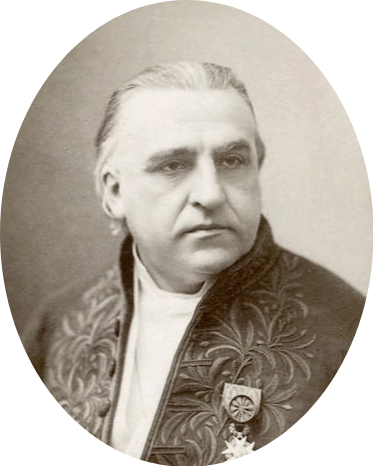
\includegraphics[width=.20\textwidth]{pic/Jean-Martin_Charcot-modified.png}
			\caption{J.-M. Charcot (1825-1893), \href{https://fr.wikipedia.org/wiki/Jean-Martin_Charcot\#/media/Fichier:Jean-Martin\_Charcot.jpg}\\
				{Wikipédia}.}
		\end{figure}
					\begin{itemize}
			\small
			\item père de la neurologie moderne
			\item contributions et influences : 
			\begin{itemize}
				\footnotesize
				\item hystérie, \og{}Parkinson\fg{}, \textsc{SLA}$\dots$
				\item Freud, de la Tourette, Babinski$\dots$
			\end{itemize}
			\item héritage scientifique vivant

			
			%			\item Fonds Charcot sur SorbonNum\footnote{\url{https://patrimoine.sorbonne-universite.fr}}
		\end{itemize}
	\end{columns}

\end{frame}


\subsection[Contexte et importance de l'étude]{Contexte et importance de l'étude}

\begin{frame}{Études des circulations culturelles et scientifiques}
	\centering
	\resizebox{1\textwidth}{!}{ 
		\begin{tikzpicture}[
			node distance=3cm and 2.5cm,
			box/.style={draw, rounded corners, fill=white, align=center, text width=6cm, font=\Large, inner sep=10pt},
			central/.style={draw, rounded corners, fill=yellow!70, text width=3.5cm, font=\LARGE\bfseries, align=center, inner sep=12pt},
			medical/.style={draw, rounded corners, fill=pink!30, text width=5cm, font=\Large, align=center, inner sep=10pt},
			science/.style={draw, rounded corners, fill=blue!60, text width=6cm, font=\Large, align=center, inner sep=10pt},
			label/.style={font=\Large\bfseries, fill=magenta!80, text=white, rounded corners, inner sep=5pt, align=center, text width=7cm},
			edge from parent/.style={draw, thick, -{Stealth}}
			]
			
			% Top label
			\node[label] at (0, 6) {Humanités numériques};
			
			% Central "Circulations" node
			\node[central] (circulations) at (0, 0) {Circulations};
			
			% Boxes in the top row
			\node[box] (images) at (-6, 3.4) {\textbf{Pensée scientifique} \\ Claude Bernard \\ (\cite{riguet2018impact})};
			\node[box] (manuscripts) at (6, 3.4) {\textbf{Manuscrits} \\ \textit{Katabase} \\ (\cite{gabay2021katabase})};
			
			% Boxes in the middle row
			\node[box] (scientific) at (-8, 0) {\textbf{Écrits littéraires} \\ Première Modernité \& HN (\cite{campanini2022circulation})};
			\node[box] (entities) at (8, 0) {\textbf{Réemplois textuels} \\ \textit{ModERN} \\ (\cite{fedchenko2024recherche})};
			
			% Boxes in the bottom row
			\node[box] (allusions) at (-7, -4) {\textbf{\OE{}uvres d'art} \\ \textit{Visual Contagions} \\ (\cite{joyeux2024greater})};
			\node[box] (reuse) at (7, -4.3)
			{\textbf{Impact des entités} \\ \textit{Rankingdom} \\ (\cite{abdallah2025rankingdom})}; 
			
			% Medical discourse box
			\node[medical] (medical) [below=of circulations, yshift=0.5cm] {\textbf{Concepts scientifiques} \\ Projet Charcot \\ (\cite{petkovic2023circulation})};
			
			
			% Science history box (renommé pour éviter conflit)
			\node[label, fill=blue!80, text width=5cm, anchor=north east] at (-8, -9) {Histoire des sciences};
			\node[science, below=of medical, text width=7cm, fill=white, yshift=0.3cm] (sciencebox) {\cite{broussolle2012} \\ \cite{tasca2012women} \\ \cite{bogousslavsky2014mysteries} \\ \cite{teive2022thomas} \\ \cite{camargo2023}};
			
			% Right label
			\node[label, fill=blue!80, text width=5cm, anchor=north west] at (8, -9) {Impact de Charcot};
			
			% Edges to central node
			\draw[edge from parent, out=180, in=0] (circulations.west) -- (scientific.east);
			\draw[edge from parent, out=0, in=180] (circulations.east) -- (entities.west);
			\draw[edge from parent] (circulations.north west) -- (images.south);
			\draw[edge from parent] (circulations.north east) -- (manuscripts.south);
			\draw[edge from parent] (circulations.south west) -- (allusions.north);
			\draw[edge from parent] (circulations.south east) -- (reuse.north);
			\draw[edge from parent] (circulations.south) -- (medical.north);
			\draw[edge from parent] (sciencebox.north) -- (medical.south);
			
		\end{tikzpicture}
	}
\end{frame}


\subsection[Objectifs de la recherche]{Objectifs de la recherche}

\begin{frame}{Double objectif}
	%	\begin{figure}
		%		\centering
		%		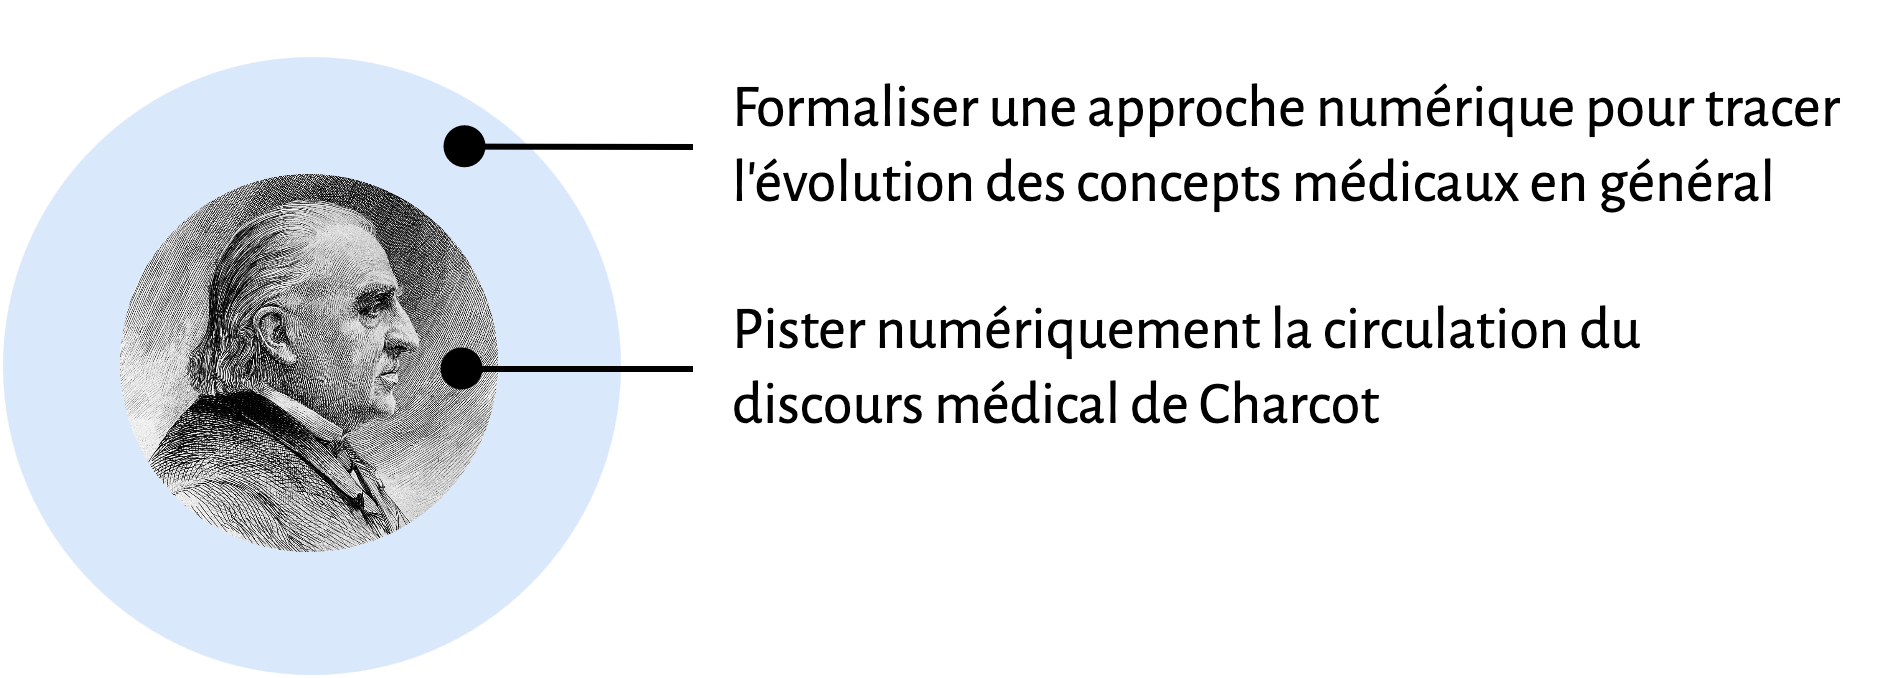
\includegraphics[width=1\textwidth]{pic/objectif_double.png}
		%		%\caption{}
		%	\end{figure}
	%	
	%	\begin{variableblock}{}{bg=white,fg=RubineRed}{bg=green,fg=red}
		%		\centering
		%		%Comment mesurer l'impact de Charcot sur son réseau scientifique ?
		%		Quels sont les concepts médicaux introduits ou transmis par Charcot qui ont eu un impact sur son réseau scientifique ?
		%	\end{variableblock}
	%	
	%	%{\footnotesize ensembles de mots liés par leur sémantique, traitant d'un domaine commun, p. ex. neurologie.}
%	Enjeu de recherche : comment les savoirs scientifiques ont été transmis la littérature médicale du \textsc{XIX}\ieme{} et \textsc{XX}\ieme{} siècle.
	\begin{tikzpicture}
		% Cercle bleu de fond
		\fill[orange!20] (0,0) circle (2.0);
		
		% Image de Charcot dans un cercle
		\node[anchor=center, circle, inner sep=0pt, minimum size=5cm, path picture={
			\node at (path picture bounding box.center){
				\includegraphics[width=2.5cm]{pic/charcot\_profil-modified.png}
			};
		}] at (0,0) {};
		
		% Points noirs
		\fill (1.1,1.1) circle (3pt);
		\fill (1.0,-0.5) circle (3pt);
		
		% Lignes
		\draw[thick] (1.1,1.1) -- (2.2,1.1);
		\draw[thick] (1.0,-0.5) -- (2.2,-0.5);
		
		% Textes (avec taille réduite et text width pour retour à la ligne)
		\node[anchor=west, align=left, text width=6cm, font=\small] at (2.3,1.1) {
			Formaliser une approche numérique pour tracer l'évolution des concepts médicaux en général
		};
		
		\node[anchor=west, align=left, text width=6cm, font=\small] at (2.3,-0.5) {
			Pister numériquement la circulation des concepts médicaux associés à Charcot
		};
		
	\end{tikzpicture}
	
%\textcolor{blue}{*} : 
%	\begin{block}{}
%				\centering
%				%Comment mesurer l'impact de Charcot sur son réseau scientifique ?
%				\textcolor{red}{Quels concepts médicaux associés à Charcot ont-ils eu un impact significatif sur son réseau\textcolor{blue}{*} scientifique du point de vue computationnel ?}
%
%			\end{block}
%			\begin{flushright}
%				\footnotesize
%				\textcolor{blue}{*} élèves, collègues et successeurs $\rightarrow$ collaborateurs
%			\end{flushright}
			
%	\begin{block}{}
%		Est-il possible de mesurer l'impact de Charcot sur son réseau* scientifique en s’appuyant sur les termes scientifiques qu'il a employés ?
%	\end{block}
\begin{enumerate}
	\item définir le terme \textit{concept scientifique} du point de vue de \textsc{TAL}
	\begin{itemize}
		\item concept ? idée ? terme ? mot ? mot-clé ? entité nommée ?
	\end{itemize}
	\item comment des concepts circulent d’une discipline à une autre
	\begin{flushright}
		\small
		\citep[p.~331]{landais2014frederic}
	\end{flushright} 
%	\item mesurer l'impact de Charcot sur l'histoire des neurosciences à travers les termes scientifiques qu'il a employés et qui ont été repris par son réseau scientifique.
\end{enumerate}


\end{frame}



\section[Problématique et hypothèses]{Problématique et hypothèses}
\subsection[Question de recherche]{Question de recherche}

\begin{frame}{Problématique principale}
	%\justifying 

	\begin{block}{Évaluer l’influence de Charcot \textit{via} les termes repris dans son réseau}
					\centering
					\textcolor{black}{Quels concepts médicaux associés à Charcot ont eu un impact computationnellement mesurable sur son réseau scientifique ?}
%	\textcolor{blue}{*}
				\end{block}

\bigskip
Concepts scientifiques en \textsc{TAL} :
\begin{itemize}
	\item termes candidats ou entités nommées (\textsc{EN}) propres à un domaine ;
	\item détectables par des patrons linguistiques (morpho-syntaxiques) ;
	\item ancrage référentiel : valeur sémantique particulière à leur contexte ;
	\item pertinence élevée selon les métriques de pondération des termes.
\end{itemize}		
\begin{flushright}
\small
\citep[pp.~1-2]{omrane2011poids}: 
\end{flushright}		
				
\end{frame}

%\subsection[Question de recherche]{Question de recherche}

\subsection[Hypothèses formulées]{Hypothèses formulées}
\begin{frame}{Hypothèses formulées}
	\begin{enumerate}
		\item 	Le texte comme point d'entrée pour étudier les tendances de la circulation des idées à l'aide des caractéristiques structurelles.
			\begin{flushright}
			\small
			\parencite[p.~2]{milia2023}
		\end{flushright}
		
		\item Certains termes médicaux associés à Charcot ont été repris de manière significative dans les écrits de son réseau scientifique.
		
		\item Chronologie d'une locution : indice de croissance de l'impact.
			\begin{figure}[h] % Use [H] to force the figure to stay in place
			\begin{itemize}
				\item évolution de la fréquence des termes au sein des deux corpus\footnote{\url{https://obtic.huma-num.fr/obvie/charcot/?view=corpus}}
				\item ex. : convergence entre des termes : fin \textsc{XIX}\ieme{}, début \textsc{XX}\ieme{} s.
				%		\begin{itemize}
					%				\item \textit{ppm} : nombre d’occurrences par million de mots 
					%		\end{itemize}
			\end{itemize}
			\centering
			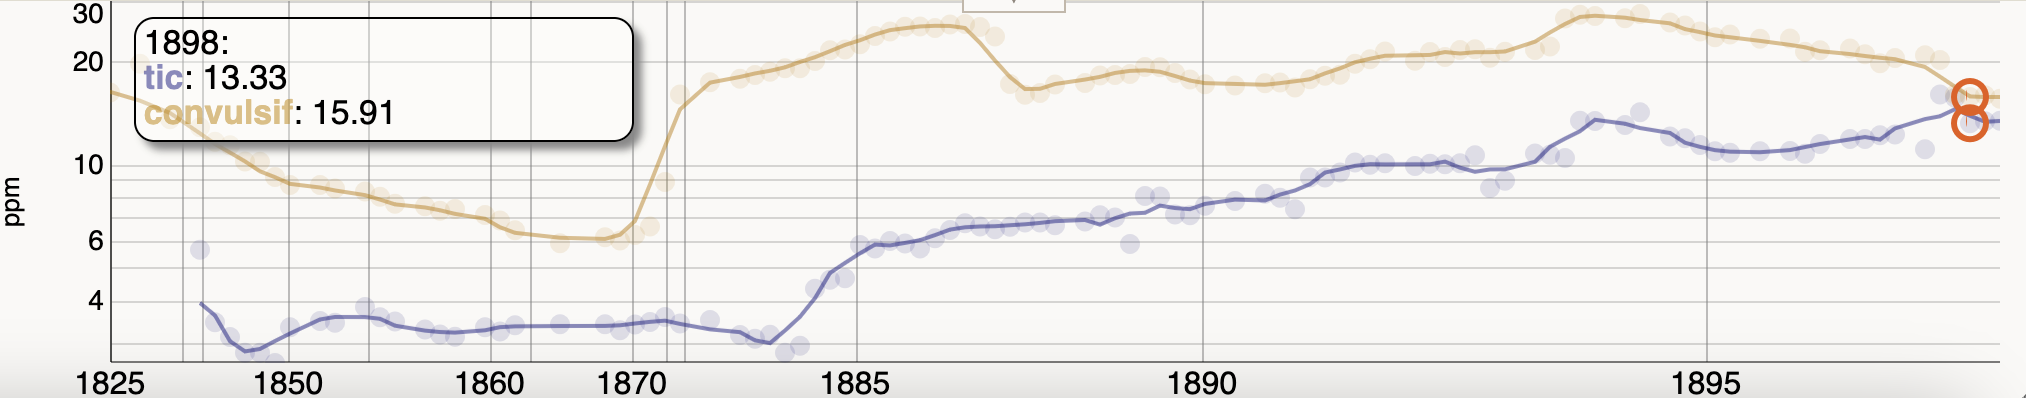
\includegraphics[width=\linewidth]{pic/tics_convulsifs.png}
			\caption{Chronologie de la fréquence du terme \textit{tic convulsif}.}
			\label{fig:ling_out_TAL}
		\end{figure}
	\end{enumerate}

	
%	\begin{block}{\begin{enumerate}
%
%		\end{enumerate}}
%	\end{block}
\end{frame}

%\begin{frame}{Chronologie d'une locution : indice de croissance de l'impact ?}
%	\begin{figure}[h] % Use [H] to force the figure to stay in place
%		\begin{itemize}
%			\item évolution de la fréquence des termes au sein des deux corpus\footnote{\url{https://obtic.huma-num.fr/obvie/charcot/?view=corpus}}
%			\item convergence entre des termes : fin \textsc{XIX}\ieme{}, début \textsc{XX}\ieme{} s.
%			%		\begin{itemize}
%				%				\item \textit{ppm} : nombre d’occurrences par million de mots 
%				%		\end{itemize}
%		\end{itemize}
%		\centering
%		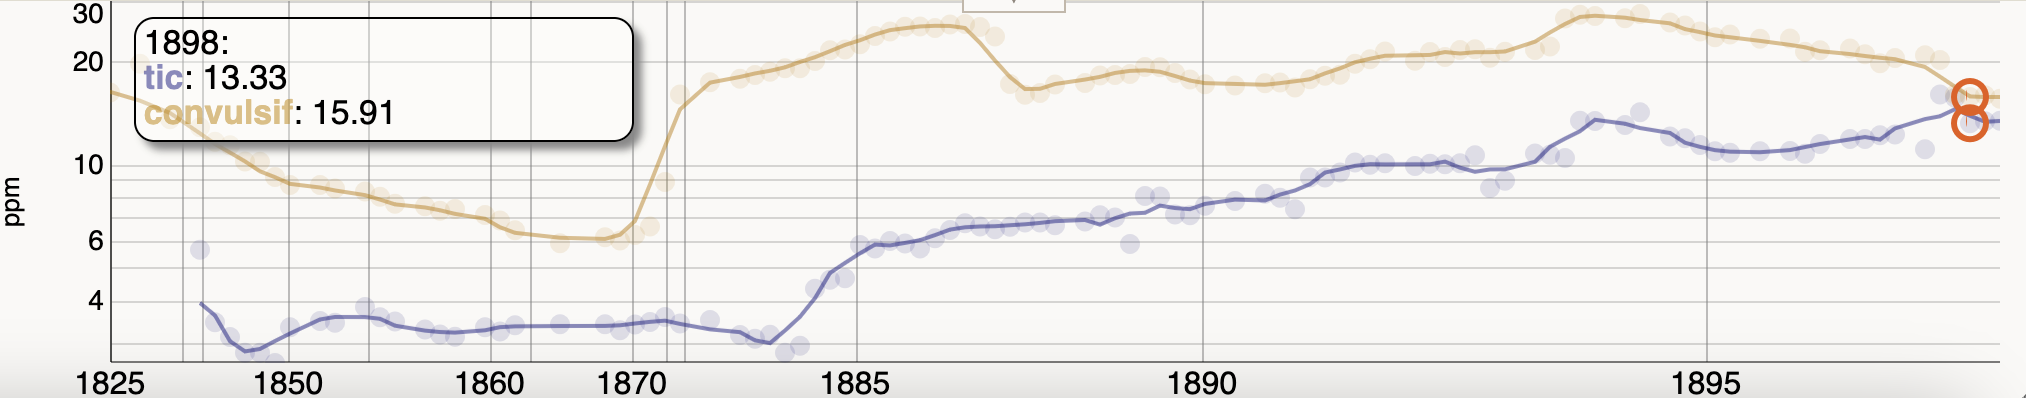
\includegraphics[width=\linewidth]{pic/tics_convulsifs.png}
%		\caption{Chronologie de la fréquence du terme \textit{tic convulsif}.}
%		\label{fig:ling_out_TAL}
%	\end{figure}
%	
%	\begin{figure}[h]
%		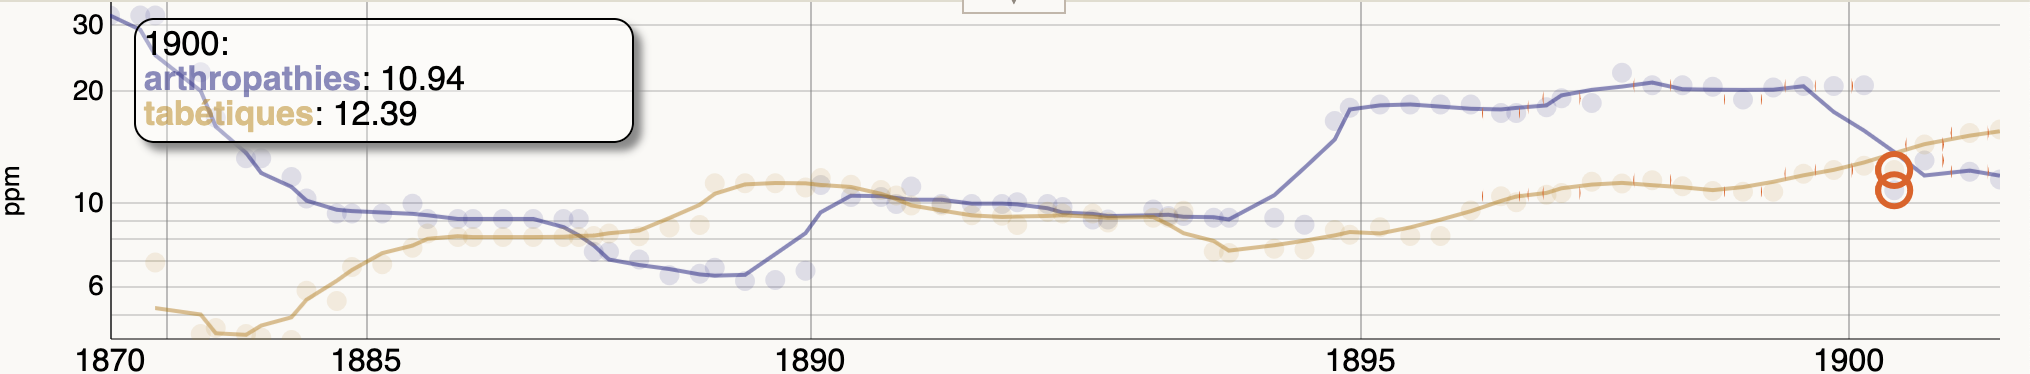
\includegraphics[width=\linewidth]{pic/arthropathies_tabetiques.png}
%		\caption{Chronologie de la fréquence du terme \textit{arthropathies tabétiques}.}
%		\label{fig:ling_out_TAL}
%	\end{figure}
%\end{frame}



\section{Extraction de la terminologie}

\subsection[Méthodes de collecte de donnée]{Méthodes de collecte de données}

\begin{frame}{Fonds Charcot\footnote{\url{https://patrimoine.sorbonne-universite.fr/collection}}}
	
{
	\setbeamercolor{block body}{bg=white}
	\setbeamercolor{block title}{bg=blue}
	
	\begin{block}{SorbonNum\\
			\footnotesize{Bibliothèque de Sorbonne Université (\textsc{BSU})}}
		201 documents XML OCRisés (sans post-correction)
	\end{block}
}
%\begin{itemize}
%    \item \textrm{Charcot} : textes rédigés par Charcot
%    \item \textrm{Autres} : textes rédigés par les membres de son réseau scientifique
%\end{itemize}
\begin{table}[!ht]
	\centering
		
		\resizebox{\textwidth}{!}{  
	\begin{tabular}{|c|r|r|r|r|r|r|r|}
		\hline 
	
		\rowcolor{yellow!30}
		Corpus & \multicolumn{1}{c|}{Docs} & \multicolumn{1}{c|}{Tokens\footnote{\url{https://spacy.io/models/fr\#fr_core_news_lg}}} & \multicolumn{1}{c|}{\%} & \multicolumn{1}{c|}{Types} & \multicolumn{1}{c|}{Lemmes} & \multicolumn{1}{c|}{Diversité} & \multicolumn{1}{c|}{Mémoire (Mo)} \\
		\hline
%		\begin{tabular}[c]{@{}c@{}}\textrm{Charcot}\\ \scriptsize{textes rédigés par Charcot}\end{tabular}
		
		 Charcot\textcolor{blue}{*} & 68 & 15 025 612 & 38,27 & 1 147 371 & 809 611 & 7,64 & 130,9\\
		\hline
%		\multicolumn{8}{|l|}{\small \textcolor{blue}{*} textes rédigés par Charcot} \\
%		\begin{tabular}[c]{@{}c@{}}\textrm{Autres}\\ \scriptsize{textes rédigés par les membres} \vspace{-0.15cm} \\ \scriptsize{de son réseau scientifique}\end{tabular}  
\hline
		Autres\textcolor{blue}{**}   & 133 & 24 232 207 & 61,73 & 1 773 538 & 1 218 074 & 7,32 & 179,6 \\ \hline
%		\multicolumn{8}{|l|}{\small \textcolor{blue}{**} textes rédigés par les membres de son réseau scientifique} \\
		\hline
		\textbf{Total} & \textbf{201} & \textbf{39 257 819} & \textbf{100} & \textbf{2 920 909} & \textbf{2 027 685} & \textbf{14,96} & \textbf{310,5} \\
%		\textbf{Total} & \textbf{201} & \textbf{31 979 479} (100\%)\\
		\hline
	\end{tabular}
}
	\caption{Description du corpus d'étude.
		%    \footnote{\tiny{\url{https://patrimoine.sorbonne-universite.fr/collection/Fonds-Charcot}}}
	}
	\label{tab:my_label}
\end{table}

{\small \textcolor{blue}{*} textes rédigés par Charcot \\
	{\small \textcolor{blue}{**} textes rédigés par son réseau scientifique}}
\end{frame}

\begin{frame}{Distribution des ouvrages du fonds Charcot}
	Entre 1825 et 1934. 
	\begin{itemize}
		\item corpus \textrm{Charcot} : fin \textsc{XIX}\ieme{}-début \textsc{XX}\ieme{} s. (1881-1907)
		\item corpus \textrm{Autres} : période plus longue (1825-1934)
	\end{itemize}
	
		\begin{figure}[h]
		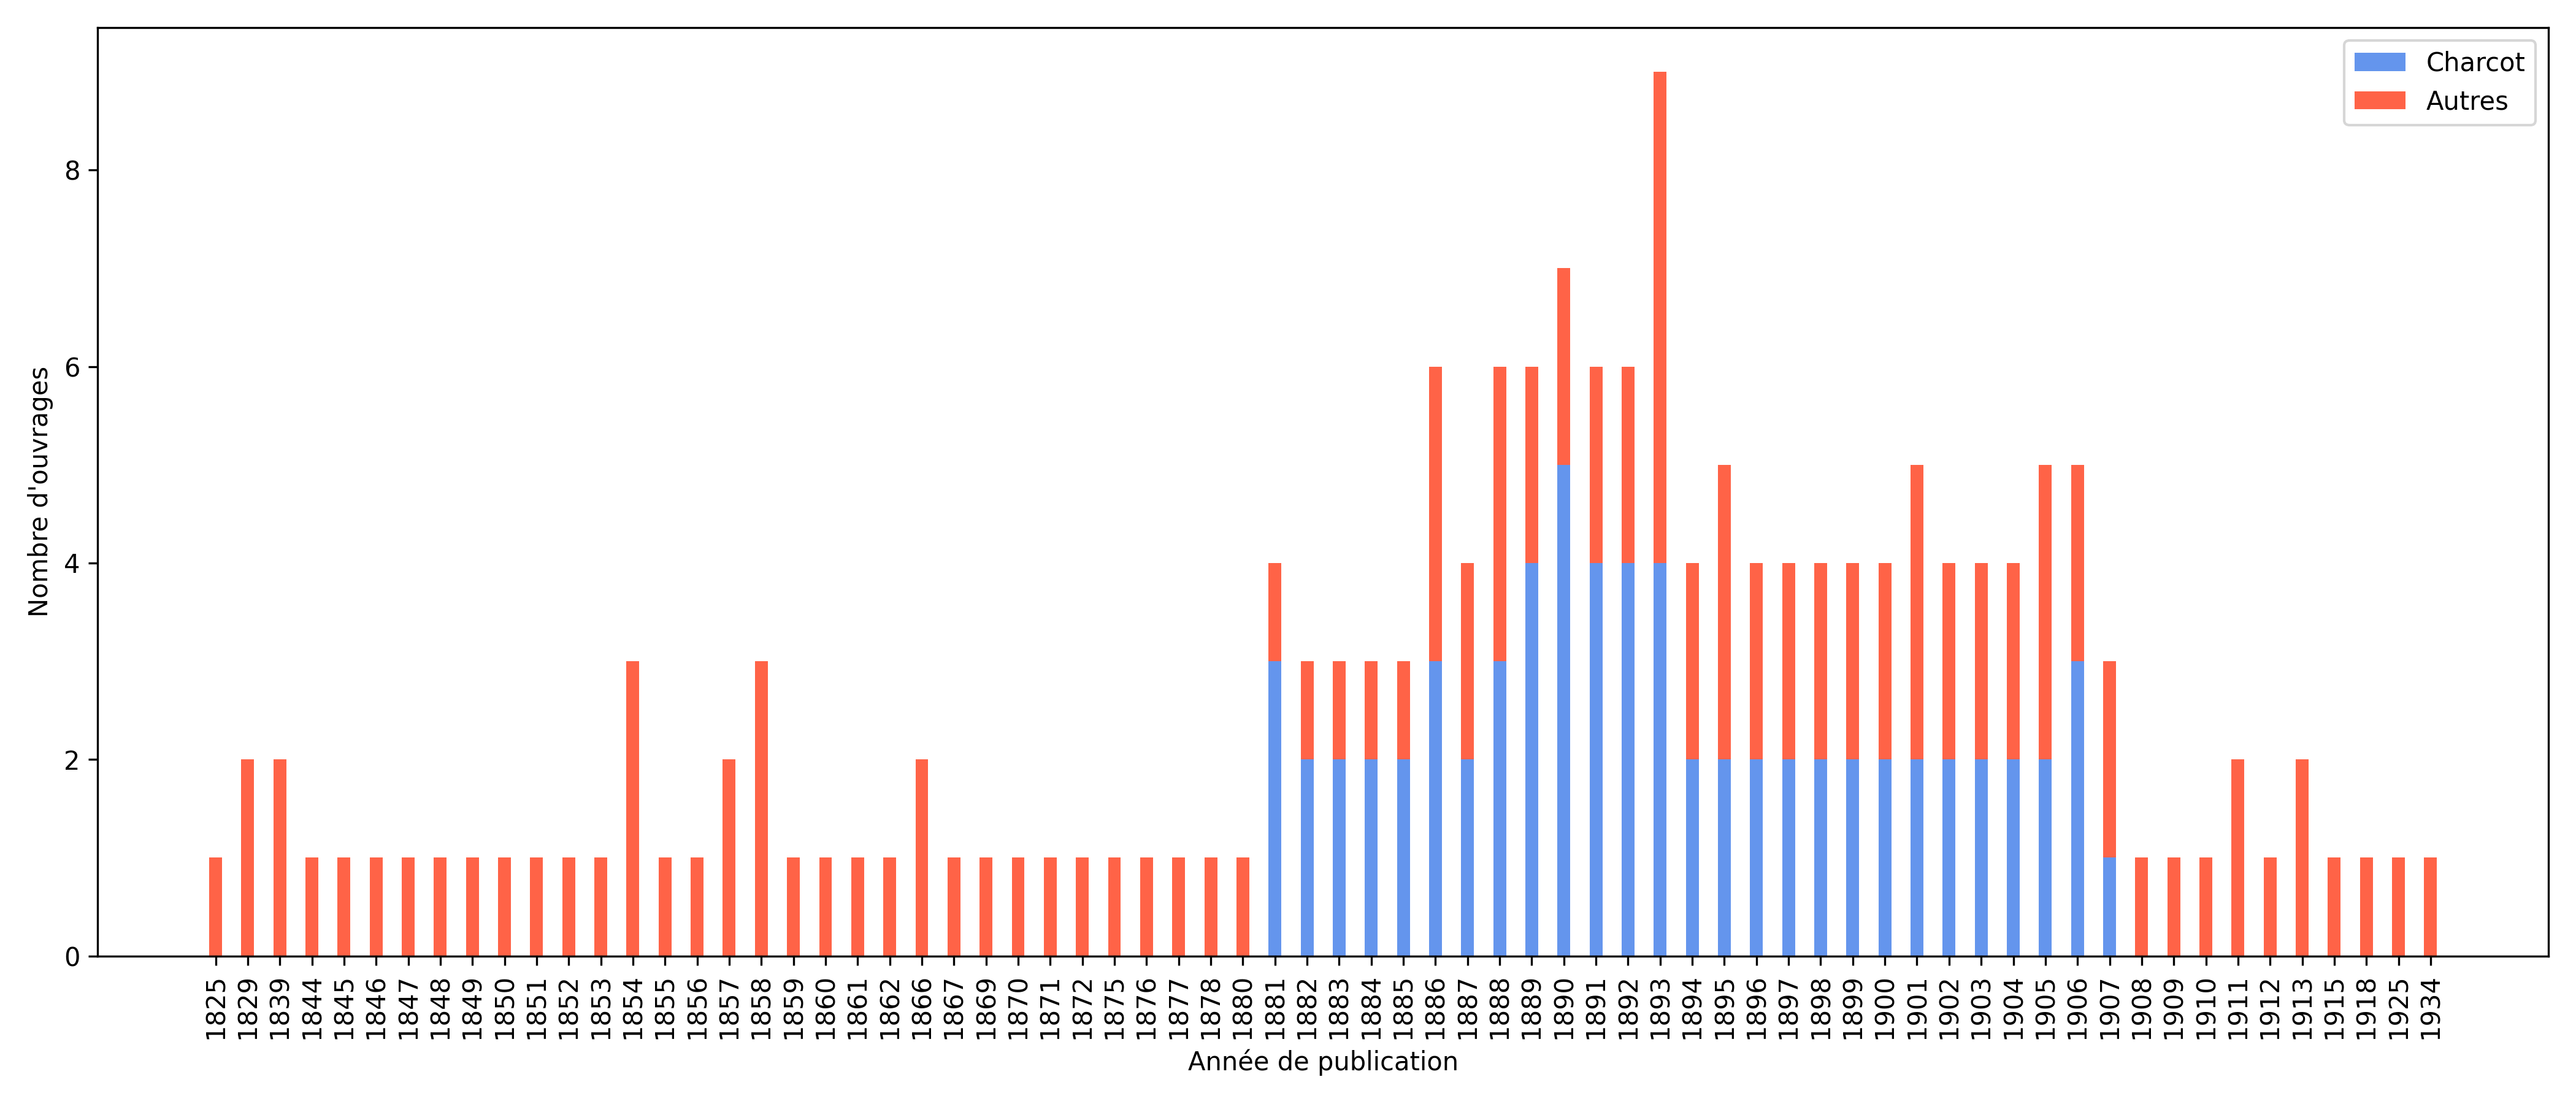
\includegraphics[width=\linewidth]{pic/distribution_ouvrages.png}
		\caption{Répartition des ouvrages constituant les corpus \og{}Charcot\fg{} et \og{}Autres\fg{} par année.}
		\label{fig:ling_out_TAL}
	\end{figure}
\end{frame}
\subsection[\textit{Design} de la recherche]{\textit{Design} de la recherche}

\begin{frame}{Formalisation de l'approche}
	\begin{itemize}
%		\item extraction terminologique
		\item comparaison des résultats avec la liste des concepts (vérité terrain)
%				\item prise en compte des synonymes des termes
%		\begin{itemize}
%			\item ex. \textit{paralysie agitante} $\rightarrow$ \textit{maladie de Parkinson} 
%		\end{itemize}
		\item recenser le score le plus élevé sur le terme ou sur son synonyme
	\end{itemize}
	\begin{figure}[h]
		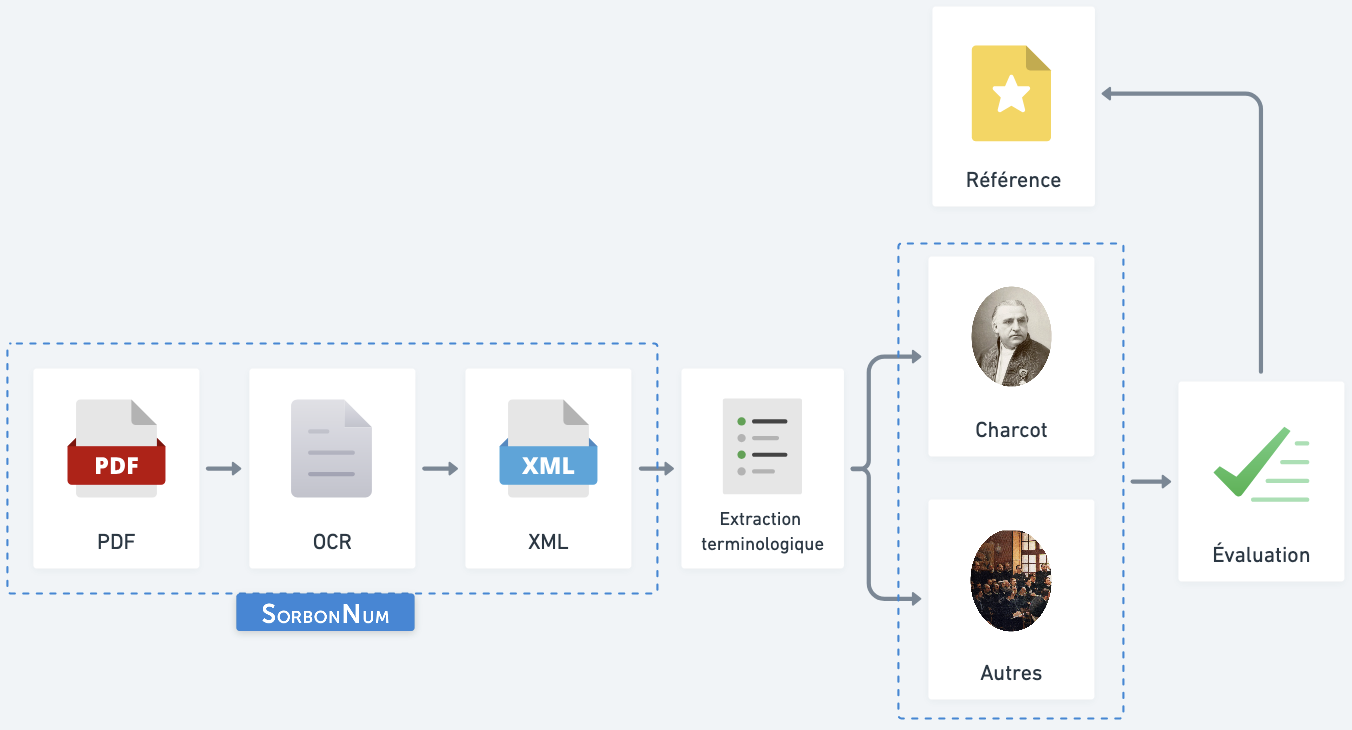
\includegraphics[width=\linewidth]{pic/formalisation_approche.png}
		\caption{\textit{Pipeline} pour pister la circulation des termes médicaux associés à Charcot.}
		\label{fig:ling_out_TAL}
	\end{figure}
\end{frame}

\begin{frame}{Liste des concepts médicaux -- vérité terrain}
	Extraction semi-automatique des termes en lien avec Charcot.\\{\scriptsize\url{https://github.com/ljpetkovic/Charcot\_circulations/tree/main/concepts}}
	
	\begin{figure}[!htb]
		\centering
		\begin{minipage}{.5\textwidth}
			\centering
			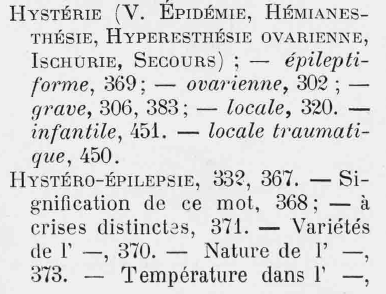
\includegraphics[width=0.6\linewidth, height=0.3\textheight]{pic/concepts-pdf}
			\caption{Index des termes \parencite{charcot1892oeuvres}.}
			\label{fig:prob1_6_2}
		\end{minipage}%
		\begin{minipage}{.5\textwidth}
			\centering
			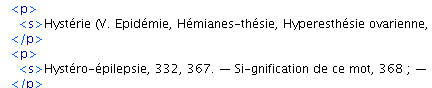
\includegraphics[width=1\linewidth, height=0.15\textheight]{pic/concepts-xml}
			\caption{Concepts médicaux, document XML.}
			\label{fig:prob1_6_1}
		\end{minipage}
	\end{figure}
	\begin{figure}[!htb]
		\centering
		\begin{minipage}{.5\textwidth}
			\centering
			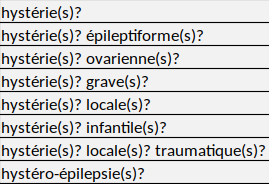
\includegraphics[width=0.6\linewidth, height=0.25\textheight]{pic/concepts-csv}
			\caption{Liste finale des concepts médicaux.}
			\label{fig:prob1_6_2}
		\end{minipage}%
		\begin{minipage}{.6\textwidth}
			\centering
			\begin{enumerate}
				\setcounter{enumi}{0}
				\item entre \texttt{<s>} et \texttt{,-(} (regex)
				\item sans termes génériques (\textit{os}, \textit{peau})
				\item prise en compte des sg. / pl. (regex)
			\end{enumerate}
		\end{minipage}
	\end{figure}
\end{frame}


\begin{frame}{Enrichissement de la liste des concepts}
	\begin{center}
		Termes \underline{inventés} par Charcot :
	\end{center}
	\begin{table}[h]
			\small
	\begin{tabular}{rl}
	
		nom traditionnel & nom moderne / synonyme \\ 		\hline
		\bolder{paralysie agitante} & maladie de Parkinson\\
		\bolder{ataxie locomotrice progressive} & \textit{tabes dorsalis}\\
		\bolder{arthropathies tabétiques} & arthropathie de Charcot\\
%		\bolder{trépidation épileptoïde du pied}  & clonus\\
		\bolder{sclérose latérale amyotrophique} & maladie de Charcot / Lou Gehrig\\
		\bolder{idée(s) fixe(s)}, \bolder{maladie des tics} &  syndrome de Tourette\\
		$\dots$
%		\bolder{mouvements involontaires}  & 	chorées, athétose\\
%		\bolder{incapacité d'être debout / de marcher} & astasie-abasie\\
%		\bolder{atrophie musculaire progressive} & maladie Charcot-Marie-Tooth
	\end{tabular}
\end{table}
	\medskip
	\begin{center}
			$\neq$ Termes \underline{transmis} par Charcot :
	\end{center}
	
	
	
		\small
		\begin{tabular}{rl}
			\textcolor{deepblue}{\textbf{athétose}} &  mouvements involontaires \\
			 \textcolor{deepblue}{\textbf{hystérie}} &  névrose \\ \textcolor{deepblue}{\textbf{épilepsie}} &  attaques convulsives \\ \textcolor{deepblue}{\textbf{hypnose}}  &  transe \\ \textcolor{deepblue}{\textbf{sclérose en plaques disséminées}} &
			  sclérose multiple
		\end{tabular}
		
			\begin{flushright}
			\scriptsize
			(\citealp{walusinski,camargo2023})
		\end{flushright}

	
	
\end{frame}



\subsection[Outils et techniques utilisées]{Outils et techniques utilisées}
\begin{frame}{Approches comparées}
%	Méthodes classiques \textit{vs.} celles de l'état de l'art.
	\begin{enumerate}
		\item \textcolor{deepblue}{\textbf{\texttt{TermSuite}}} \footnote{\url{https://github.com/ljpetkovic/Charcot_TermSuite}} \citep{cram2016terminology}
		\begin{itemize}
			\item linguistique, à base de règles $\rightarrow$ TD-IDF
		\end{itemize} 
		\item \textcolor{deepblue}{\textbf{TF-IDF, BM25}}\footnote{\url{https://github.com/ljpetkovic/Charcot_circulations}} \citep{robertson1976relevance}  
		\begin{itemize}
			\item statistique
		\end{itemize}
		\item \textcolor{deepblue}{\textbf{\textit{PatternRank}}} \citep{schopf2022}\footnote{\url{https://github.com/ljpetkovic/Seminaire_doctoral_ObTIC_130325/blob/main/0_main.pdf}}
		\begin{itemize}
			\item apprentissage profond
			\item \texttt{keybert} + \texttt{keyphrase-vectorizers}
			\item utilisation des étiquettes POS
		\end{itemize} 
	\end{enumerate}
	
	\begin{block}{\vspace*{-0.6mm}}
		Traitements effectués en local (1,2) et \textit{via} la plateforme MeSU\footnote{\url{https://sacado.sorbonne-universite.fr/fr/plateforme-mesu/}} (3).
		\begin{itemize}
			\item appliqués à tout le corpus
		\end{itemize}
	\end{block}
	
\end{frame}

%\subsection[Échantillon et population étudiée]{Échantillon et population étudiée}
%\begin{frame}{Extraction des phrases-clés}
%\og{}\textcolor{deepblue}{Phrases-clés}\fg{}, angl. \textit{keyphrases}
%\begin{itemize}
%\item séquences de plusieurs mots (ex. \textit{sclérose latérale amyotrophique})
%\item reflètent plus précisément le contexte sémantique du texte \\\small{$\neq$ mots-clés, angl. \textit{keywords} : unigrammes de mot (ex. \textit{sclérose})}
%\end{itemize}
%\bigskip
%%\centering
%%Extraction de \og{}phrases-clés\fg{} (angl. \textit{keyphrases})
%%\\~\\
%%\begin{block}{Extraction de phrases-clés}
%%\justifying
%%Processus de \underline{sélection} automatique d'un petit ensemble de phrases les plus pertinentes à partir d'un texte donné \citep{schopf2022}.
%%\end{block}
%%\begin{block}{Prédiction de phrases-clés}
%%\justifying
%%Processus de \underline{génération} des phrases-clés qui résument parfaitement un document donné \citep{xie2023}.
%\begin{columns}[t,onlytextwidth]
%\column{.45\textwidth}
%\textcolor{violet}{Extraction}
%\justifying
%
%Processus de \underline{sélection} automatique d'un petit ensemble de phrases les plus pertinentes à partir d'un texte donné.
%\vspace{-0.2cm}
%\begin{flushright}
%\small{\citep{schopf2022}}
%\end{flushright} 
%\column{.45\textwidth}
%\textcolor{violet}{Prédiction}
%\justifying
%
%Processus de \underline{génération} des phrases-clés qui résument parfaitement un document donné.
%\vspace{0.3cm}
%\begin{flushright}
%\small{\citep{xie2023}}
%\end{flushright}
%\end{columns}%Extraction de phrases-clés
%%
%%Processus de \underline{sélection} automatique d'un petit ensemble de phrases les plus pertinentes à partir d'un texte donné \citep{schopf2022}.
%%
%%\begin{block}{Prédiction de phrases-clés}
%%\justifying
%%Processus de \underline{génération} des phrases-clés qui résument parfaitement un document donné \citep{xie2023}.
%%\end{block} 
%\end{frame}

\begin{frame}{Extraction des phrases-clés : méthode \texttt{keybert}}
	\begin{enumerate}
		\small
		\item entrée : un document
		\item tokénisation du document en phrases-clés candidates (PCC)
		\item génération des plongements du doc. et des PCC par un modèle de langage
		\item calcul de la similarité cosinus entre le document et les PC
	\end{enumerate}
	\begin{figure}
		\centering
		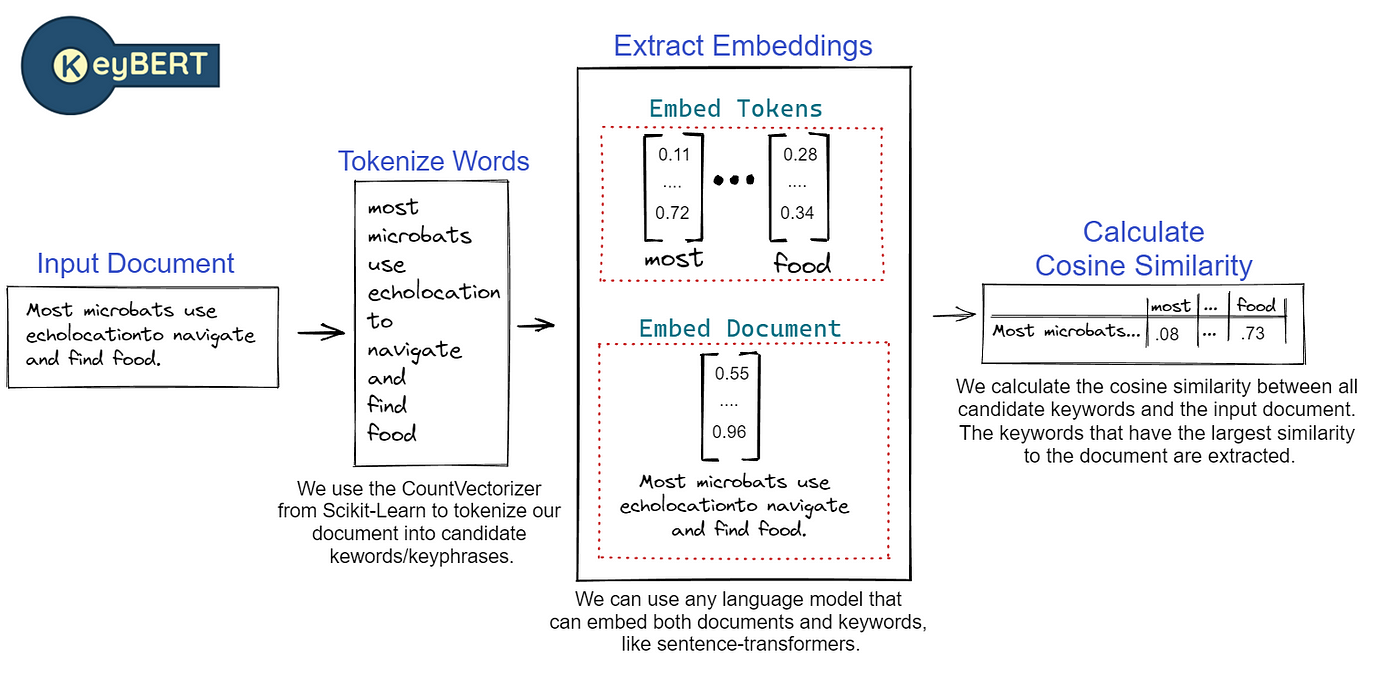
\includegraphics[width=80mm,scale=0.5]{pic/keybert.png}
		\caption{\textit{Pipeline} de la librairie \texttt{keybert} \citep{grootendorst2020keybert}.}
		\label{fig:enter-label}
	\end{figure}
\end{frame}

\begin{frame}{Extraction des phrases-clés : méthode \textit{PatternRank}\\
		\quad \quad \quad\ \quad \quad \quad \quad \quad \quad \quad \ \ \ \ \ \small{Librairie \texttt{keyphrase-vectorizers}}}
	%\begin{itemize}
	%\item extraction des phrases-clés non-supervisée
	%\item exploite des modèles de langues pré-entraînés + parties du discours
	%\end{itemize}
	\begin{enumerate}
		\small
		\item entrée : un seul document texte tokenisé
		\item étiquetage des tokens avec les balises du partie du discours (POS)
		\item sélection des tokens selon le motif POS $\rightarrow$ phrases-clés candidates (PCC)
		\item génération des plongements du doc. et des PCC par un modèle de langue
		\item calcul des similarités cosinus entre ces deux types de plongements +  \\classement des PCC par ordre décroissant
		\item extraction des \textit{N} PC les plus représentatives
	\end{enumerate}
	\begin{figure}
		\centering
		\includegraphics[width=110mm,scale=0.5]{pic/patternrank\_workflow.png}
		\caption{\textit{Workflow} de la méthode \textit{PatternRank} \citep{schopf2022}.}
		\label{fig:enter-label}
	\end{figure}
	\notecite{schopf2022}
\end{frame}



\section{Résultats}
\subsection[Présentation des résultats principaux]{Présentation des résultats principaux}
	% Tableau Charcot
\begin{frame}{Domaine impactant dans les écrits de Charcot : \textbf{hystérie}}
	\vspace*{-3mm}
	\begin{table}[h]
		\resizebox{\textwidth}{!}{%
			\centering
			\begin{tabular}{|l|r|r|r|r|r|}
				\hline
				\multicolumn{1}{|c|}{\textbf{Terme}}
				&	\multicolumn{1}{c|}{\textbf{TF-IDF} (\textit{TermSuite})} & 	\multicolumn{1}{c|}{\textbf{TF-IDF}} & 	\multicolumn{1}{c|}{\textbf{BM25}} & 	\multicolumn{1}{c|}{\textit{\textbf{PatternRank}}} & \multicolumn{1}{c|}{\textbf{Moyenne}} \\
				\hline
				\textit{maladie de Parkinson} & NA  & 0,2478 & 0,2397  & 0,7926 &  0,3200 \\
				\textit{ataxie locomotrice progressive} & 0,1981  & 0,4114 & 0,2313 &  0,7912 & 0,408 \\
				\textit{arthropathies tabétiques} & 0,4424 & 0,1655 & 0,337 & 0,8050 & 0,4375 \\
				\textit{trépidation épileptoïde du pied} & 0,0379 & 0,2581 & 0,053 & 0,7581 & 0,2768 \\
				\textit{sclérose en plaques disséminées} & NA & 0,2935 & 0,4812 & 0,7611 & 0,3840 \\
				\textit{tremblement} & NA & 0,2712 & 0,0213 &  0,7834 & 0,2690 \\
				\textit{nystagmus} & NA & 0,2142 & 0,0488 & 0,7683 & 0,2578 \\
				\textit{embarras parole} & NA & 0,0724 & 0,9143 & 0,8159 & 0,4507 \\
				\textit{sclérose latérale amyotrophique} & NA & 0,3287 & 0,1152 & 0,7514 & 0,2988 \\
				\textit{tics convulsifs} & 0,0670 & 0,2273 & 0,1696 & 0,8073 & 0,3178\\
				\textit{atrophie musculaire progressive} & 0,1161 & 0,2321 & 0,0797 & 0,7874 & 0,3038 \\
				%		\textit{abasie} & NA & NA & 0,0445 & 0,3325\\
				\textit{aphasie} & 0,1722 & 0,345 & 0,0289 & 0,7824 & 0,3321 \\
				\textit{astasie-abasie} & 0,1281 & 0,7022 & 0,1912 & 0,7891 & 0,4527 \\
				\textit{athétose} & NA & 0,226 & 0,0797 & 0,7910 & 0,2742\\
				\textit{chorées} & 0,1593 & 0,1933 & 0,0213 & 0,8030 & 0,2942 \\
				\rowcolor{yellow!30}\textit{hystérie} & 0,6892 & 0,5407 & 0,0213 & 0,8194 & \bolder{0,5177} \\
				\textit{épilepsie} & 0,0062 & 0,534 & 0,0213 & 0,8170 & 0,3446 \\
				\textit{hypnose} & 0,0311 & 0,4294 & 0,0994 & 0,7955 & 0,3389\\
				\textit{systématisation de l'organisation de la moëlle épinière} & NA & 0 & 0 & NA & 0 \\
				\textit{localisations cérébrales} & NA & 0,27 & 0,0943 & 0,7493 & 0,2784 \\
				\hline
			\end{tabular}
		}
		\caption{Les scores de pertinence pour les termes de référence à partir du corpus \og{}Charcot\fg{}.}
	\end{table}
	{\small Moyenne pour tous les termes combinés : 0,3280}
\end{frame}


% Tableau Autres

\begin{frame}{Domaine impactant dans les écrits des Autres : \textbf{syndrome de Tourette}}
	
	
	\begin{table}[h]
		\resizebox{\textwidth}{!}{%
			\centering
			\begin{tabular}{|l|r|r|r|r|r|}
				\hline
				\multicolumn{1}{|c|}{\textbf{Terme}}
				&	\multicolumn{1}{c|}{\textbf{TF-IDF} (\textit{TermSuite})} & 	\multicolumn{1}{c|}{\textbf{TF-IDF}} & 	\multicolumn{1}{c|}{\textbf{BM25}} & 	\multicolumn{1}{c|}{\textit{\textbf{PatternRank}}} & \multicolumn{1}{c|}{\textbf{Moyenne}} \\
				\hline
				\textit{maladie de Parkinson} & 0,05 & 0,0775 & 0,333 & 0,7936 & 0,3135  \\
				\textit{ataxie locomotrice progressive} & 0,32 & 0,0386 & 0,4877 &  0,7431 & 0,3974 \\
				\textit{arthropathies tabétiques} & 0,33 & 0,0934 & 0,4928 & 0,7506 & 0,4167 \\
				\textit{trépidation épileptoïde du pied} & 0,0198 & 0,1227 & 0,2919 & 0,7597 & 0,2985 \\
				\textit{sclérose en plaques disséminées} & NA  & 0,178 & 0,8089 & NA & 0,2467 \\
				\textit{tremblement} & NA & 0,1686 & 0,0362 & 0,7683 & 0,2432 \\
				\textit{nystagmus} & 0,0243 & 0,1326 & 0,146 & 0,7474 & 0,2626 \\
				\textit{embarras parole} & NA & NA & 0,0018 & 0,9347 & 0,2341 \\
				\textit{sclérose latérale amyotrophique} & NA & 0,044 & 0,6586 & NA & 0,1757 \\
				\rowcolor{yellow!30}\textit{tics convulsifs} & NA & 0,1293 & 0,8385 & 0,8331 & \bolder{0,4502}\footnote{Le score le plus élevé parmi les termes \textbf{inventés} par Charcot $\neq$ \textit{hypnose}.} \\
				\textit{atrophie musculaire progressive} & 0,40 & 0,1118 & 0.3489 & 0,8053 & 0,4165 \\
				%		\textit{abasie} & NA & NA & 0,0445 & 0,3325\\
				\textit{aphasie} & 0,0587 & 0,2245 & 0,1334 & 0,7960 & 0,3031 \\
				\textit{astasie-abasie} & NA & 0,0478 & 0,3565 & 0,7375 & 0,2855 \\
				\textit{athétose} & NA & 0,2029 & 0,274 & 0,8068 & 0,3209 \\
				\textit{chorées} & NA & 0,1336 & 0,0701 & 0,8047 & 0,2521 \\
				\textit{hystérie} & 0,2724 & 0,3711 & 0,0442 & 0,8018 & 0,3723 \\
				\textit{épilepsie} & NA & 0,164 & 0,0247 & 0,8199 & 0,2521 \\
				\textit{hypnose} & 0,3543 & 1 & 0,2922 & 0,7738 & 0,6050 \\
				\textit{systématisation de l'organisation de la moëlle épinière} & NA & NA & NA & 0,7550 & 0,1888 \\
				\textit{localisations cérébrales} & 0,43 & 0,034 & 0,3017 & 0,8090 & 0,3937 \\
				\hline
			\end{tabular}
		}
		\caption{Les scores de pertinence pour les termes de référence à partir du corpus \og{}Autres\fg{}.}
	\end{table}
	{\small Moyenne pour tous les termes combinés : 0,3214}
\end{frame}

\begin{frame}{Limitations de \texttt{keybert}}
	\danger{} manque de diversification des résultats + (non-)grammaticalité\\
	\begin{figure}[!ht]
		\centering
		\includegraphics[width=110mm,scale=0.5]{pic/termes\_keybert\_autres.png}
		\caption{Répartition des 15 termes les plus pertinents dans le corpus \og{}Autres\fg{} selon \texttt{keybert}.}
		\label{fig:enter-label}
	\end{figure}
\end{frame}

\begin{frame}{Phrases-clés \textit{hapax} partagés dans les deux corpus selon \texttt{keybert}}
	Les seuls termes partagés avec le corpus Charcot : 
	%\begin{itemize}
	%\item articulations de [\textit{sic}] épaule
	%\item paralysie faciale périphérique
	%\end{itemize}
	\begin{figure}[!ht]
		\centering
		\includegraphics[width=90mm,scale=0.5]{pic/termes\_partages\_keybert.png}
		\caption{Répartition des termes les plus pertinents dans les deux corpus selon \texttt{keybert}.}
		\label{fig:enter-label}
	\end{figure}
\end{frame}


%\begin{frame}{Termes partagés extraits avec \texttt{keyphrase-vectorizers}}
%    \begin{figure}[!ht]
	%        \centering
	%        \includegraphics[width=85mm,scale=0.5]{pic/visualisation_termes_dupliques.png}
	%        \caption{Les termes communs aux deux corpus selon \texttt{keyphrase-vectorizers}.}
	%        \label{fig:enter-label}
	%    \end{figure}
%\end{frame}

%\begin{frame}{Termes partagés | \texttt{keyphrase-vectorizers}}
%    \begin{figure}[!ht]
	%        \centering
	%        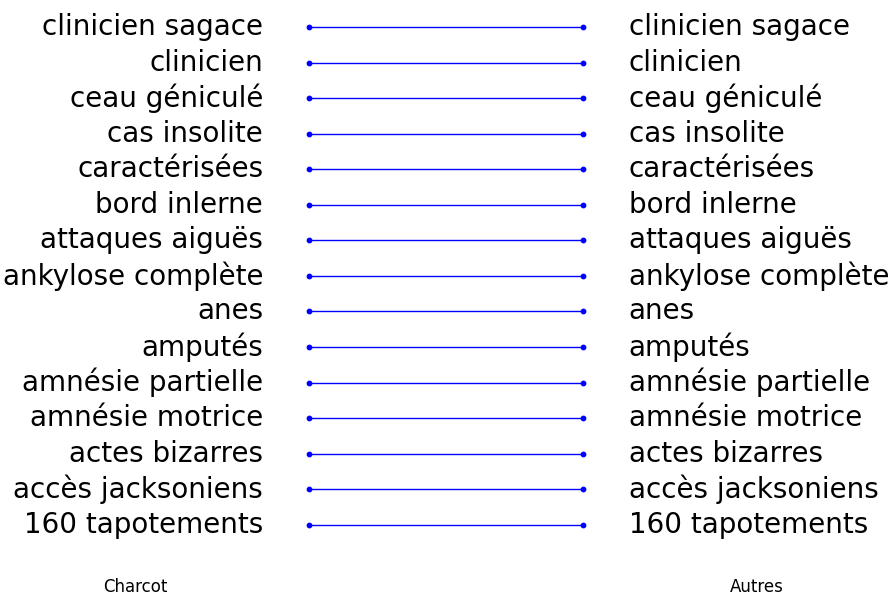
\includegraphics[width=100mm,scale=0.5]{pic/termes_partages_liens.png}
	%        \caption{Les termes communs (fréq. = 1) aux deux corpus selon \texttt{keyphrase-vectorizers}.}
	%        \label{fig:enter-label}
	%    \end{figure}
%\end{frame}

\begin{frame}{Les termes partagés les plus fréquents | \texttt{keyphrase-vectorizers}}
	\begin{figure}[!ht]
		\centering
		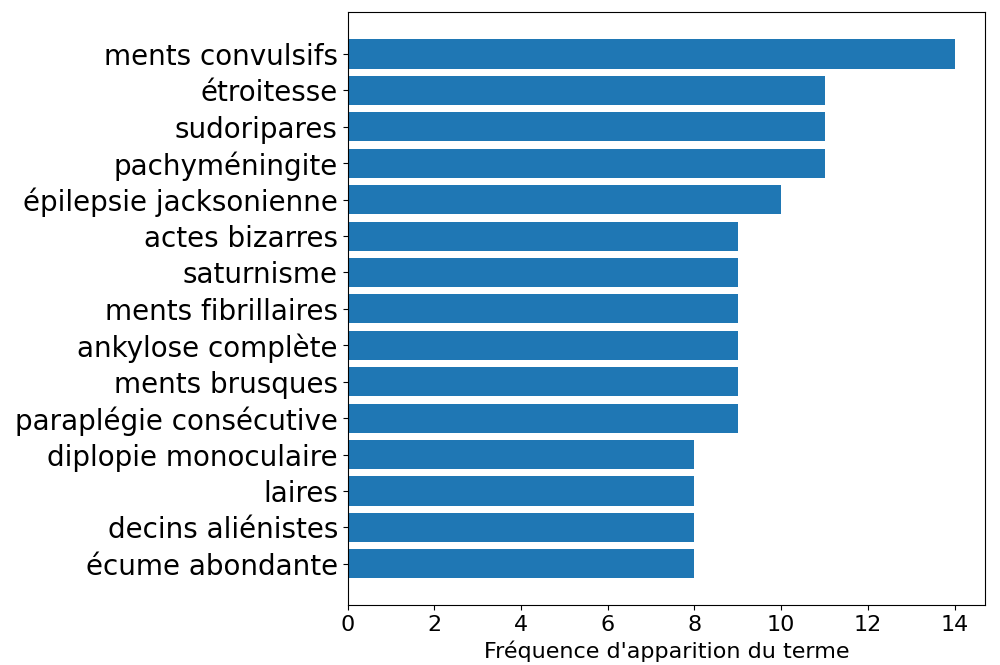
\includegraphics[width=100mm,scale=0.5]{pic/termes_partages.png}
		\caption{Les 15 termes les plus fréquents dans les deux corpus selon \texttt{keyphrase-vectorizers}.}
		\label{fig:enter-label}
	\end{figure}
\end{frame}



\begin{frame}{Analyse comparative des approches employées}
	\begin{itemize}
		\item \textit{PatternRank} valorise systématiquement les termes
		\item pas de consensus entre les métriques
		\begin{itemize}
			\item l'écart le plus petit entre eux : \textit{hypnose}
		\end{itemize}
	\end{itemize}
	\begin{figure}[h]
		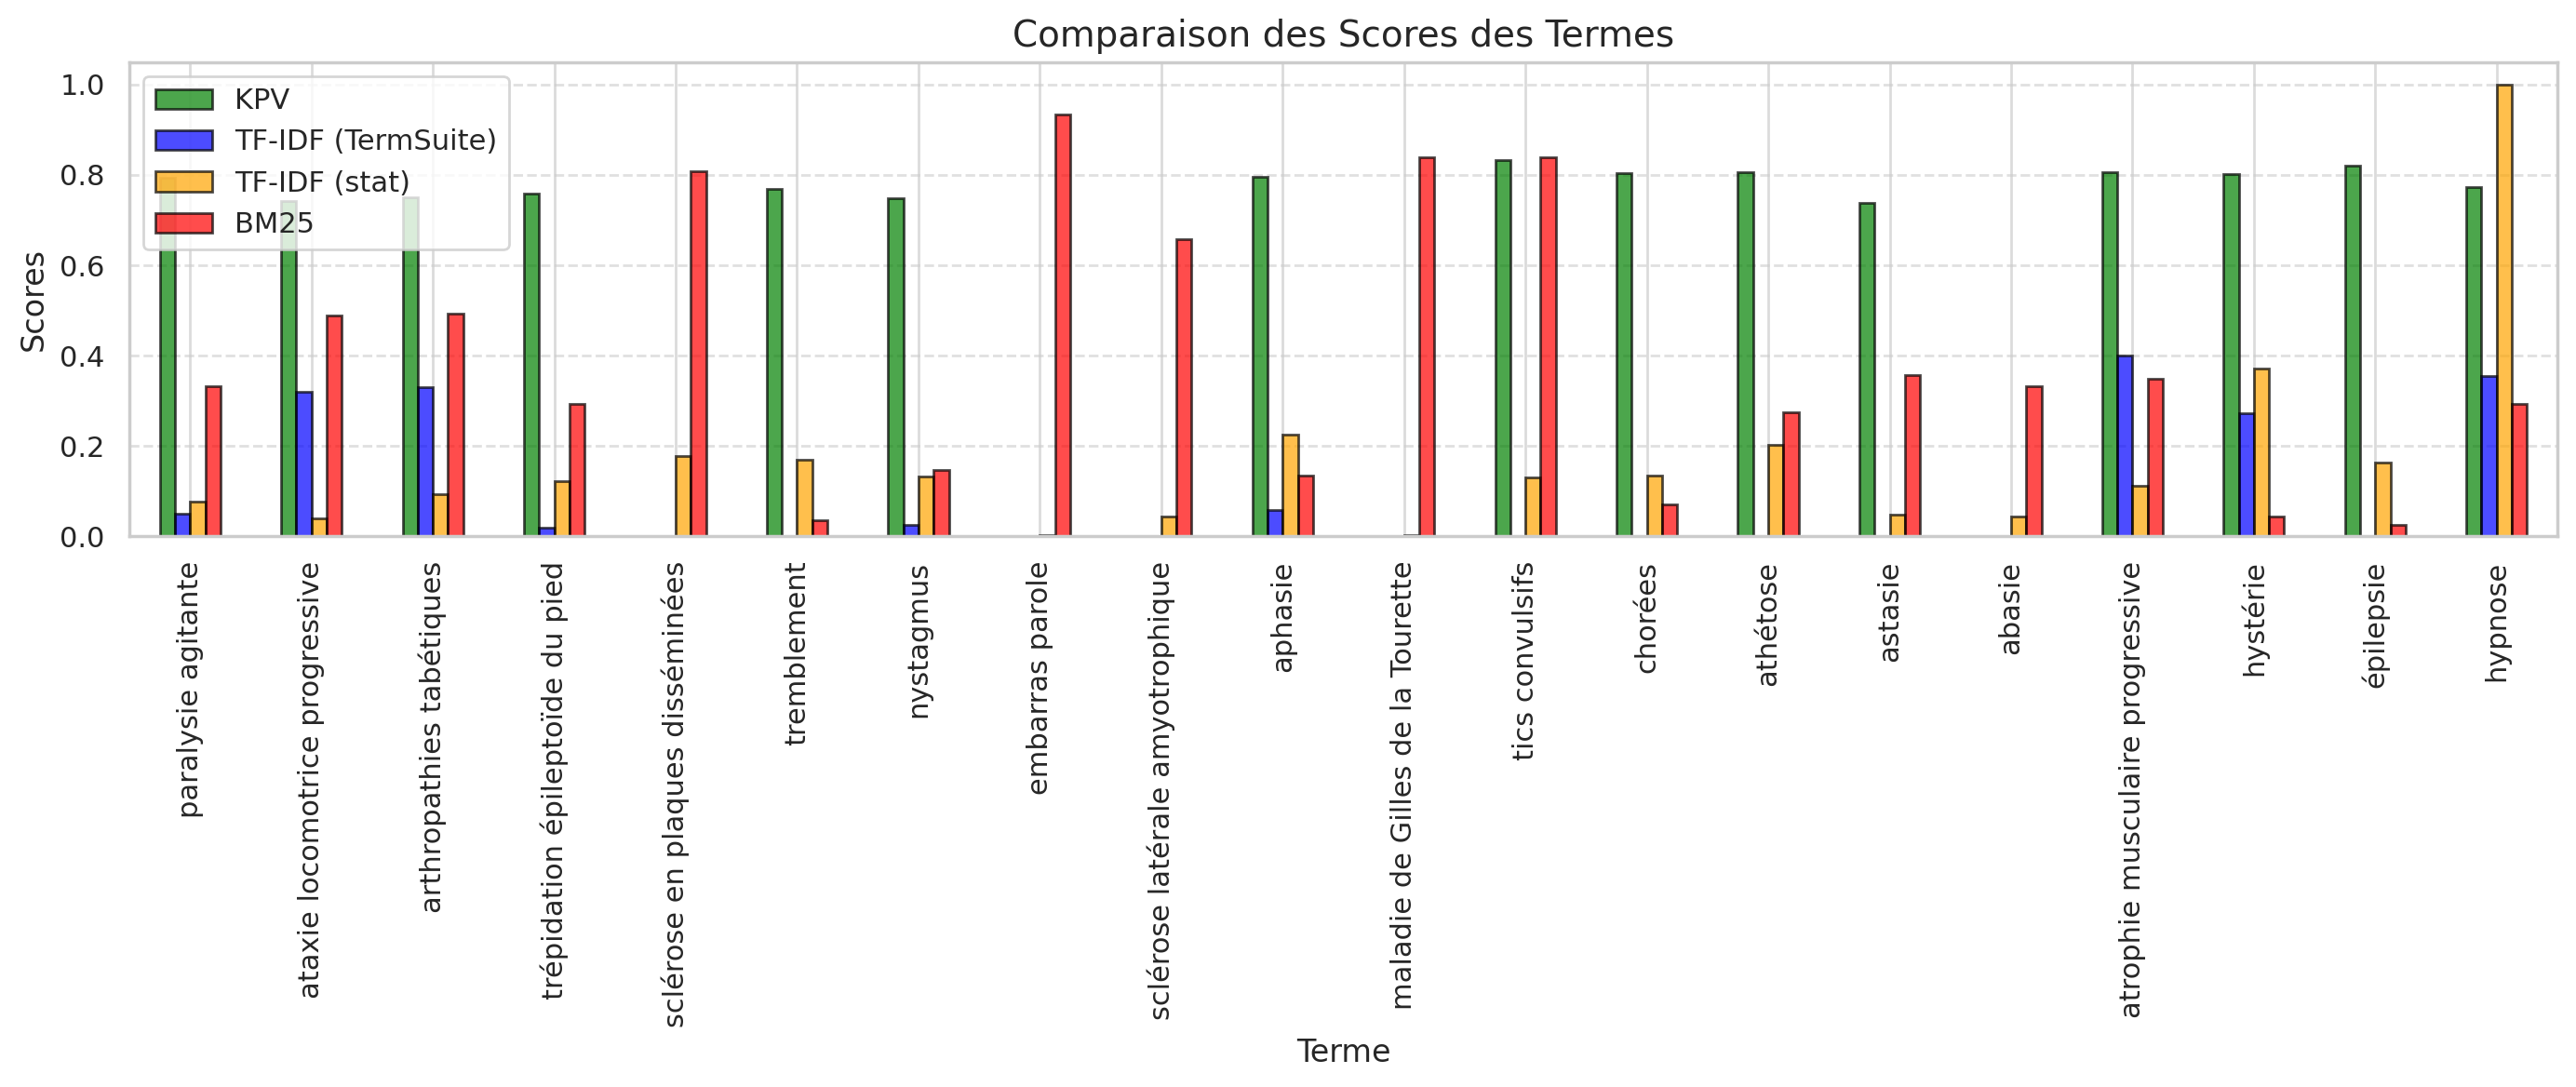
\includegraphics[width=\linewidth]{pic/termes_viz.png}
		\caption{Visualisation des scores de pertinences pour chaque terme de référence.}
		\label{fig:ling_out_TAL}
	\end{figure}
\end{frame}

%\begin{frame}{Accès à la plateforme technologique \textsc{MeSU}}
%\begin{itemize}
%\item expériences réalisées sur la plateforme \href{https://sacado.sorbonne-universite.fr/}{\textsc{MeSU}} de Sorbonne Université
%\end{itemize}
%\bigskip
%
%Les données et les scripts utilisés dans le cadre de cette étude sont disponibles sur le \href{https://github.com/ljpetkovic/JE\_IA\_HN\_030524}{dépôt GitHub}.
%\end{frame}

%\begin{frame}{Analyse comparative des approches employées}
%	\begin{itemize}
%		\item \textit{PatternRank} valorise systématiquement les termes
%		\item pas de consensus entre les métriques
%		\begin{itemize}
%			\item l'écart le plus petit entre eux : \textit{hypnose}
%		\end{itemize}
%	\end{itemize}
%	\begin{figure}[h]
%		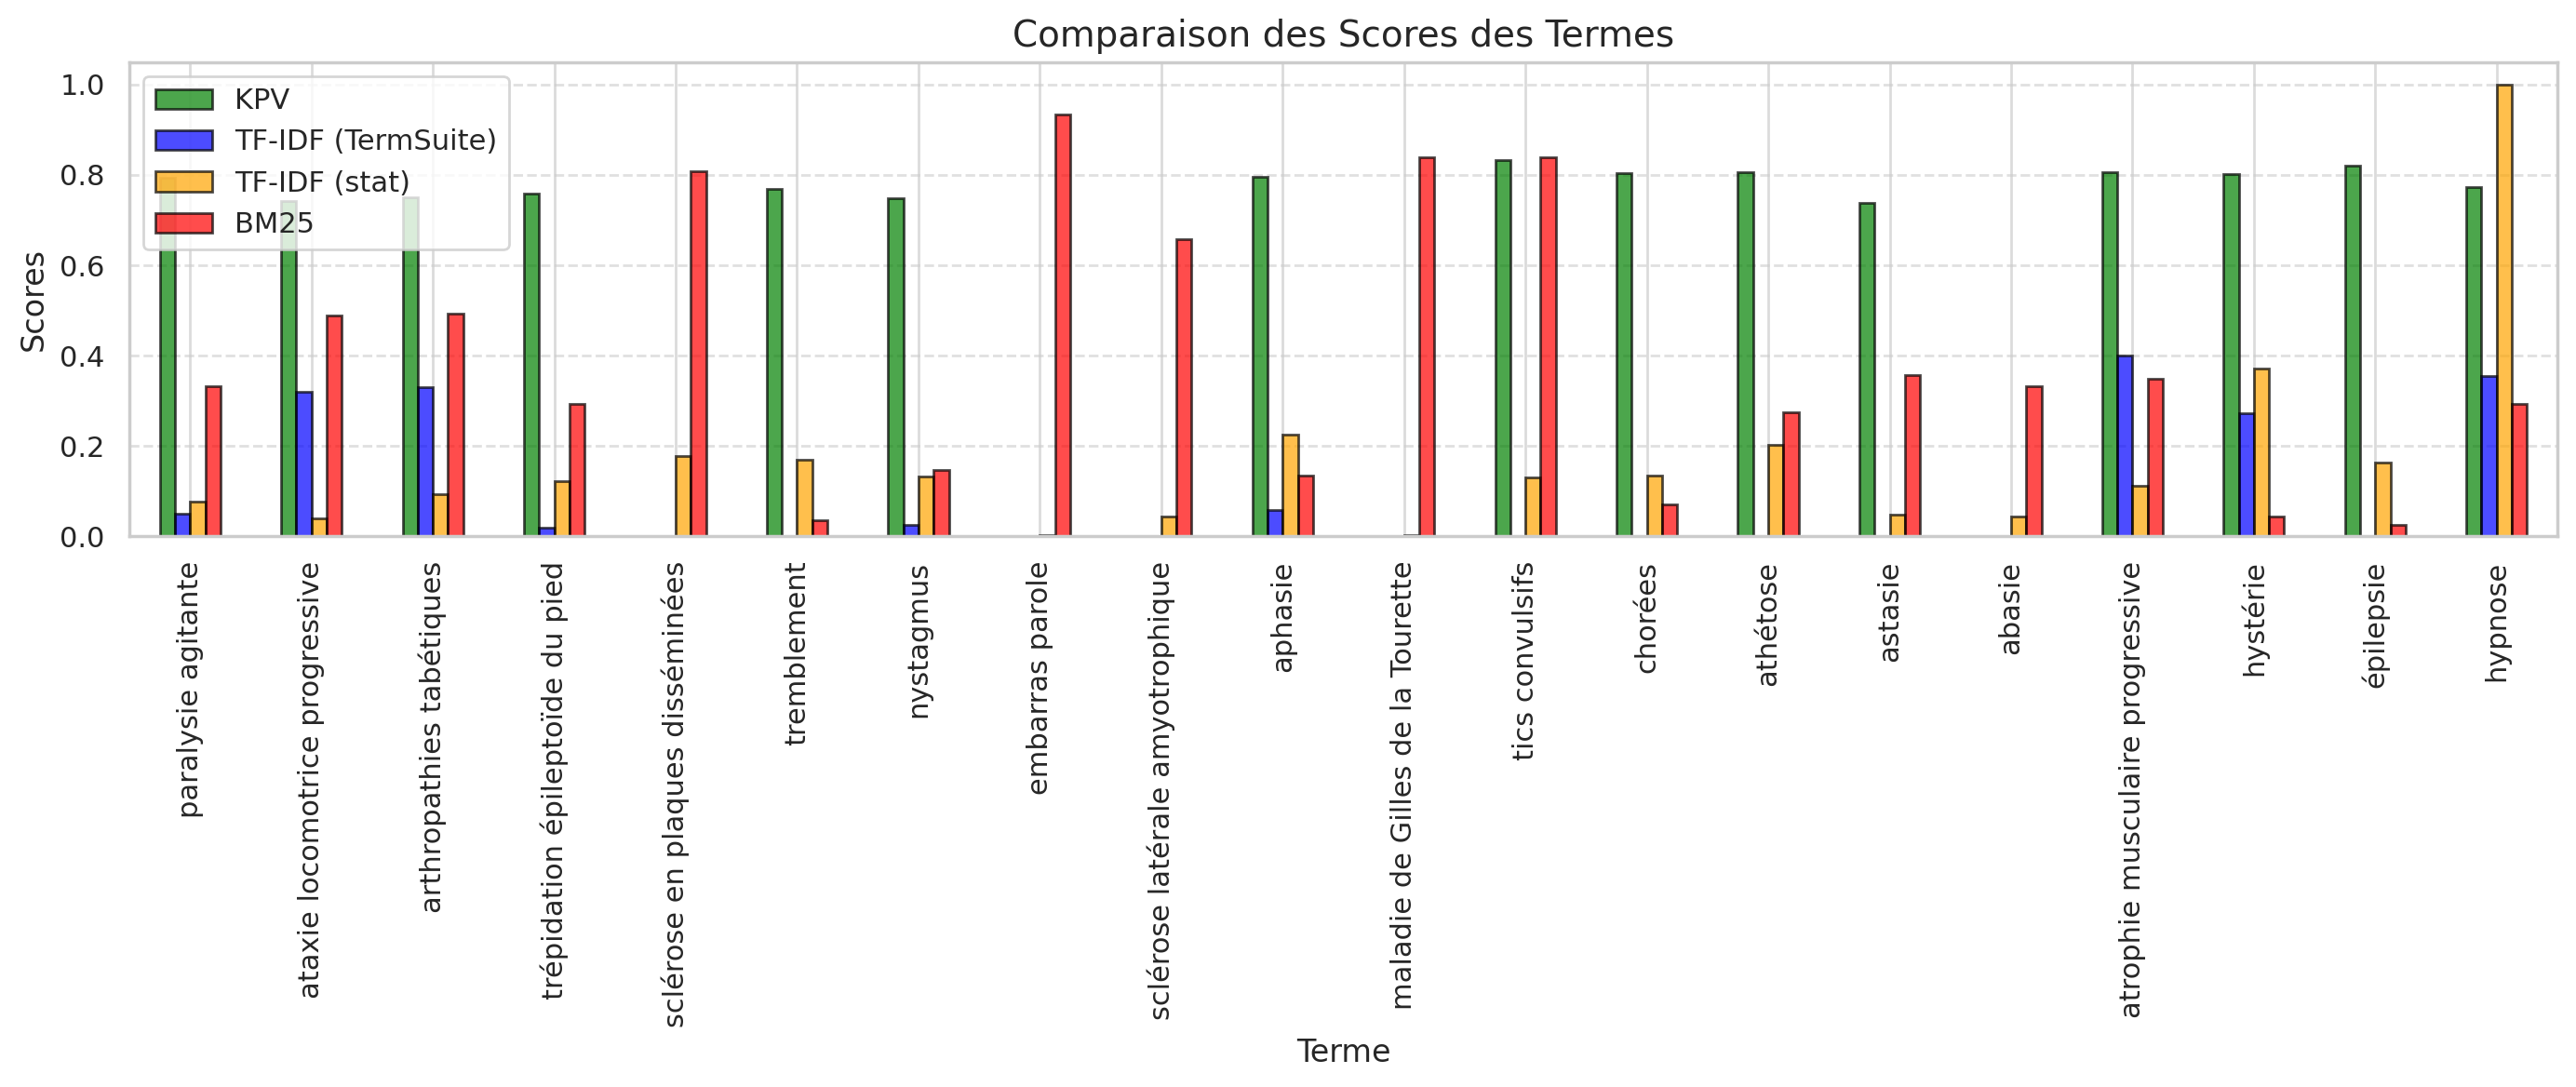
\includegraphics[width=\linewidth]{pic/termes_viz.png}
%		\caption{Visualisation des scores de pertinences pour chaque terme de référence.}
%		\label{fig:ling_out_TAL}
%	\end{figure}
%\end{frame}
\subsection[Analyse et interprétation des résultats]{Analyse et interprétation des résultats}

% analyse quali
\begin{frame}{Analyse des concordances des termes médicaux}
	Analyses effectuées dans \textsc{TXM}.
	\begin{itemize}
		\item on utilise un terme dans le contexte où on cite Charcot
		\begin{itemize}
			\item terme traditionnel (ex. \textit{paralysie agitante})
			\item synonyme ou terme relevant du champ conceptuel en question
			\begin{itemize}
%				\item ensembles de mots liés à un certain concept \citep{costachescu2024}\\
				\item \textit{pied tabétique} $\rightarrow$ forme particulière d'\textit{arthropathies tabétiques}
			\end{itemize}
		\end{itemize}
	\end{itemize}
	\begin{block}{Exemple}
		\texttt{([word = "paralysie"] [word = "agitante"] []* [word = "Charcot"] | [word = "Charcot"] []* [word = "paralysie"] [word = "agitante"]) within p}
		\begin{itemize}
			\item repérer toutes les occurrences dans un paragraphe où \textit{paralysie agitante} et \textit{Charcot} apparaissent dans n'importe quel ordre, séparés par 0 ou plusieurs mots
		\end{itemize}
	\end{block}
\end{frame}

\begin{frame}{Références à Charcot}
	
	\begin{table}
		\centering
		\resizebox{\textwidth}{!}{%
			\begin{tabular}{|l|p{10cm}|}
				\hline
				\textbf{Terme} & \textbf{Contexte} \\
				\hline
				\textit{maladie de Parkinson} & [$\dots$] \underline{paralysie agitante} que \textbf{Charcot} a eu raison de dénommer \underline{maladie de Parkinson} \\
				\hline
				\textit{ataxie locomotrice progressive} & [$\dots$] arthropathies [$\dots$] de l'\underline{ataxie locomotrice}, [$\dots$] signalées, pour la première fois, par M. \textbf{Charcot}. \\
				& [$\dots$] \underline{ataxie locomotrice progressive}, constatée par douze médecins, parmi lesquels, [$\dots$] MM. \textbf{Charcot} [$\dots$] \\
				\hline
				\textit{arthropathies tabétiques} & [$\dots$] mais personne n'avait encore décrit des cas d'\underline{arthropathie tabétique}, lorsque, en 1808, M. le professeur \textbf{Charcot} publia la première observation d'arthropathie chez un ataxique.\\
				\hline
				\textit{trépidation épileptoïde du pied} & [$\dots$] \underline{trépidation}, qui se propage parfois à tous les \underline{membres}. Ce spasme, [$\dots$] peut entraîner à sa suite des rétractions fibro-tendineuses analogues à celles que \textbf{Charcot} a décrites chez l'homme, [$\dots$] \\
				\hline
				\textit{sclérose en plaques disséminées} & [$\dots$] une combinaison de la \underline{sclérose en plaques}, bien décrite déjà par \textbf{Charcot} et Vulpian [$\dots$] \\
				\hline
			\end{tabular}
		}
		\caption{Concordance des termes médicaux faisant référence à Charcot -- corpus Autres.}
	\end{table}
\end{frame}


\begin{frame}{Références à Charcot}
	
	\begin{table}
		\centering
		\resizebox{\textwidth}{!}{%
			\begin{tabular}{|l|p{10cm}|}
				\hline
				\textbf{Terme} & \textbf{Contexte} \\
				\hline
				\textit{tremblement} & [$\dots$] \textbf{Charcot} présentait, dans son amphithéâtre, pour démontrer les caractères oscillatoires des diverses variétés de \underline{tremblements}. \\
				\hline
				\textit{nystagmus} & SCLÉROSE EN PLAQUES [$\dots$] [$\dots$], \underline{nystagmus}, [$\dots$]. La difficulté de la résoudre est d'autant plus grande qu'à côté des foyers de sclérose en plaques avec tous les caractères histologiques classiques décrits depuis \textbf{Charcot}, il y a des foyers avec une
				destruction plus ou moins complète des cylindraxes [$\dots$]\\
				\hline
				\textit{embarras parole} & Lorsqu'on se trouve en présence d'un malade ayant de l'\underline{embarras de la parole} [$\dots$] A. La réponse à la première proposition n'est nullement embarrassante, si l'on veut se rappeler ces paroles de M. le professeur \textbf{Charcot} : [$\dots$] \\
				\hline
				\textit{sclérose latérale amyotrophique} & [$\dots$] \underline{sclérose latérale amyotrophique}, maladie découverte par mon illustre maître \textbf{Charcot}. \\
				\hline
				\textit{tics convulsifs} & désignée par M. \textbf{Charcot} sous le nom de maladie des \underline{tics convulsifs} \\
				\hline
				\textit{atrophie musculaire progressive} & \textbf{Charcot} et Marie ont décrit la \og{}forme particulière d'\underline{atrophie musculaire progressive}\fg{}\\
				\hline
				\textit{aphasie} & Lorsqu'il y a, dit M. le professeur \textbf{Charcot} (1), suppression de la mémoire pour l'articulation des mots, c'est l'\underline{aphasie} motrice d'articulation ou \underline{aphasie} de Broca qui se présente.\\
				\hline
			\end{tabular}
		}
		\caption{Concordance des termes médicaux faisant référence à Charcot -- corpus Autres (suite).}
	\end{table}
\end{frame}

\begin{frame}{Références à Charcot}
	
	\begin{table}
		\centering
		\resizebox{\textwidth}{!}{%
			\begin{tabular}{|l|p{10cm}|}
				\hline
				\textbf{Terme} & \textbf{Contexte} \\
				\hline
				\textit{astasie-abasie} & [$\dots$] forme particulière d'impuissance motrice dont M. P. Blocqe a donné la
				définition suivante \og{}[$\dots$], et qu'il a désigné sous le nom expressif d'\underline{astasie} et d'\underline{abasie}. C'est là un état morbide sur lequel M. le professeur \textbf{Charcot} est	fréquemment revenu dans ses Leçons du mardi [$\dots$]\\
				\hline
				\textit{athétose} & symptôme désigné par M. W. Hammond sous le nom d'\underline{athétose} [$\dots$] M. \textbf{Charcot} a fait remarquer que cette définition était imparfaite pour les motifs suivants : [$\dots$] \\
				\hline
				\textit{chorées} & \underline{Chorée} hystérique ou rhythmique. C'est à M. le professeur \textbf{Charcot} que nous devons une exacte description de cet état pathologique. \\
				\hline
				\textit{hystérie} & C'est encore à \textbf{lui} [Charcot] que nous devons la connaissance de l'\underline{hystérie} traumatique [$\dots$] \\
				\hline
				\textit{épilepsie} & M. \textbf{Charcot} a décrit avec le plus grand soin l'\underline{épilepsie} partielle d'origine syphilitique [$\dots$] \\
				\hline
				\textit{hypnose} & Les trois états de l'\underline{hypnose} décrits par M. \textbf{Charcot} sont devenus classiques, [$\dots$] \\
				\hline
				\textit{systématisation de l'organisation de la moëlle épinière} & \underline{systématisation de la moelle}, synthèses [$\dots$]. Mais \textbf{Charcot}, on l'a vu, est, par nature, enclin à la synthèse. \\
				\hline
				\textit{localisations cérébrales} & Je vous ai montré \textbf{Charcot}, concourant pour
				la plus grosse part, à l'édification de la doctrine des \underline{localisations cérébrales}, qui est devenue quelque chose comme la préface d'une psychologie nouvelle.\\
				\hline
			\end{tabular}
		}
		\caption{Concordance des termes médicaux faisant référence à Charcot -- corpus Autres (fin).}
	\end{table}
\end{frame}

\begin{frame}{Analyse des cooccurrences}
	\begin{itemize}
		\item quels cooccurrents avec les termes médicaux ciblés ? 
		\begin{itemize}
			\item Charcot, Babinski, Necker$\dots$
		\end{itemize}
		\item recensement des résultats pour le cooccurrent : Charcot
		\item sinon, autre cooccurrent (médecin) avec l'indice le plus élevé\\
		\begin{alertblock}{Exemple}
			\texttt{[word = "athétose"]} 
			\begin{itemize}
				\item liste des cooccurrents pour le terme \textit{athétose}
			\end{itemize}
		\end{alertblock}
	\end{itemize}
\end{frame}

\begin{frame}{Analyse des cooccurrences}
	\begin{table}[h]
		\centering
		\resizebox{\textwidth}{!}{%
			\begin{tabular}{rrrrrr}
				\textbf{Terme} & \textbf{Cooccurrent} & \textbf{Fréquence} & \textbf{Co-fréquence} & \textbf{Indice} & \textbf{Distance moyenne} \\
				\hline
				maladie de Parkinson  & Charcot & 2 968 &  3 & 2 & 3,3\\
				ataxie locomotrice progressive  & Charcot & 2 968 & 3 & 2 & 5,3 \\
				arthropathies tabétiques & Charcot & 2 968 & 4 & 5 & 1,5 \\
				trépidation épileptoïde du pied & Babinski $\cdot$ Charcot &  1 134 &  8 & 12 & 4,8 \\
				sclérose en plaques disséminées & Charcot & 2 968 & 7 & 3 & 6,3 \\
				tremblement & Achard & 137 & 3 & 2 &  2,3\\
				nystagmus & Barany & 11 & 3 & 7 & 3,3\\
				embarras parole & Chervin & 41 & 8 & 17 & 4,5\\
				sclérose latérale amyotrophique & Charcot & 2 968 & 4 & 3 & 3,5 \\
				tics convulsifs & Charcot & 2 968 & 6 & 8 & 5,2 \\
				atrophie musculaire progressive & Charcot & 2 968 & 4 & 3 & 6,0 \\
				aphasie & Charcot & 2 968 & 7 & 2 & 4,0\\
				astasie-abasie & Charcot & 2 968 & 2 & 2 & 1,5 \\
				athétose & Hammond & 34 & 2 & 4 & 1,5\\
				chorées & Sydenham & 129 & 63 & 163 & 1,1 \\
				\rowcolor{yellow!30}hystérie & Charcot & 2 968 & 52 & 19 & 5,4\\
				épilepsie & Jackson & 52 & 34 & 78 & 0,2 \\
				hypnose & Braid & 567 & 14 & 12 & 4,7 \\
				systématisation de l'organisation de la moëlle épinière & NA & NA & NA & NA & NA \\
				localisations cérébrales & Charcot & 2 968 & 9 & 7 & 5,3 \\
			\end{tabular}
		}
		\caption{Analyse des cooccurrences des termes médicaux à partir du corpus Autres.}
		\label{tab:cooccurrences}
	\end{table}
	
\end{frame}

\begin{frame}{Analyse des cooccurrences}
	Absence occasionnelle de cooccurrent Charcot expliquable :
	\begin{itemize}
		\item \textit{épilepsie} : terme créé par J. H. Jackson
		\item \textit{hypnose} : terme créé par J. Braid
		\item \textit{athétose} : terme créé par W. A. Hammond
		\item \textit{chorées} : définition moderne par T. Sydenham
		\item \textit{trépidation épileptoïde du pied} : Babinski ? Vulpian? Charcot ? 			
	\end{itemize}
\end{frame}

\begin{frame}{Analyse des autres cooccurrents}
	\begin{table}
		\centering
		\resizebox{\textwidth}{!}{%
			\begin{tabular}{|l|p{10cm}|}
				\hline
				\textbf{Terme} & \textbf{Contexte} \\
				\hline
				\textit{trépidation épileptoïde du pied} (\textit{clonus}) & \textbf{On} [Babinski] le désigne alors sous la dénomination de \og{}\underline{clonus du
					pied}\fg{}, \og{}\underline{trépidation épileptoïde du pied}\fg{} \\ \hline
				\textit{tremblement} &  D'après \textbf{Charcot} et surtout d'après \textbf{Achard}, ce \underline{tremblement} aurait de certaines analogies avec le tremblement sénile, [$\dots$] \\ \hline
				\textit{nystagmus} & [$\dots$] les recherches inspirées par les
				travaux de \textbf{Barany} sur le \underline{nystagmus} provoqué indiqueraient une certaine fréquence de troubles labyrinthiques [$\dots$] \\ \hline
				\textit{embarras parole} & M. le Dc \textbf{Chervin}, [$\dots$] vient de rédiger un nouveau résumé des notions cliniques fondamentales indispensables à connaître sur quelques \underline{troubles fonctionnels de la parole} et notamment sur le bégaiement. 
				\\
				\hline
				\textit{athétose} & [$\dots$] nous avons affaire au symptôme désigné par M. W. \textbf{Hammond} sous le nom d'\underline{athétose}.\\
				\hline
				\textit{chorées} & Cependant, la \underline{chorée} de \textbf{Sydenham} présente quelques particularités sémiologiques que nous allons passer en revue.\\ \hline 
				
				épilepsie & Depuis les remarquables travaux de M. Hughlings \textbf{Jackson} sur la forme d'\underline{épilepsie} à laquelle il a attaché son nom, [$\dots$] \\ \hline
				\textit{hypnose} & Selon \textbf{Braid}, l'\underline{hypnose} est caractérisée par des phénomènes mentaux et physiques, particuliers à cette condition.\\
				\hline
			\end{tabular}
		}
		\caption{Concordance des termes médicaux faisant référence à d'autres médecins -- corpus Autres.}
	\end{table}
\end{frame}

%\begin{frame}{Cas ambigu de la \textit{trépidation épileptoïde du pied} (\textit{clonus})}
%	
%	\begin{quote}
%		\textbf{On} le désigne alors sous la dénomination de \og{}\underline{clonus du pied}\fg{}, de \og{}\underline{trépidation épileptoïde du pied}\fg{}.
%	\end{quote}
%	\begin{flushright}
%		\small
%		\parencite{babinski1934oeuvre}
%	\end{flushright}
%	
%	
%	
%	\begin{quote}
%		\small
%		[$\dots$] l'un d'eux, [$\dots$], est
%		connu en France sous le nom de \underline{trépidation provoquée},	\underline{d'épilepsie spinale provoquée}. Les auteurs allemands rappelent le phénomène du pied ‭{\underline{Fussph\oe{}nomen}}, ou encore le \underline{clonus du pied}.
%		Mais c'est là un signe qui appartient ‭à la clinique française. Dès ‭1863, [$\dots$], il ‭était journellement mis ‭à profit dans les services de la Salpêtrière, par M. \textbf{Vulpian}, par \textbf{moi-même} et par \textbf{nos ‭élèves}.
%	\end{quote}
%	
%	\begin{flushright}
%		\small
%		\parencite{brissaud1893}
%	\end{flushright}
%	%		CL\_000001\_004 (pas inclus dans le corpus Autres -.-)
%	%		\bigskip
%	%					\begin{quote}
%		%			“$\dots$ known in France under the name of \underline{provoked trepidation}, or \underline{provoked spinal epilepsy}. German writers call it the foot-phenomenon (\underline{Fussphoenomen}) or \underline{ankle clonus}. But \textbf{the discovery of this sign belongs to French clinical observers}. Since 1863$\dots$ it has been \textbf{practised} daily in the wards of La Salpêtrière \textbf{by M. Vulpian, by myself} {\normalfont[Charcot]}, \textbf{and by our pupils}.”
%		%		\end{quote}
%	%		\begin{flushright}
%		%			\small
%		%			\citep{charcot1883lectures}
%		%		\end{flushright}
%	%	
%\end{frame}

%\begin{frame}{Analyse comparative des approches employées}
%	\begin{itemize}
	%		\item \textit{PatternRank} valorise systématiquement les termes
	%		\item pas de consensus entre les métriques
	%		\begin{itemize}
		%			\item l'écart le plus petit entre eux : \textit{hypnose}
		%		\end{itemize}
	%	\end{itemize}
%\begin{figure}[h]
%	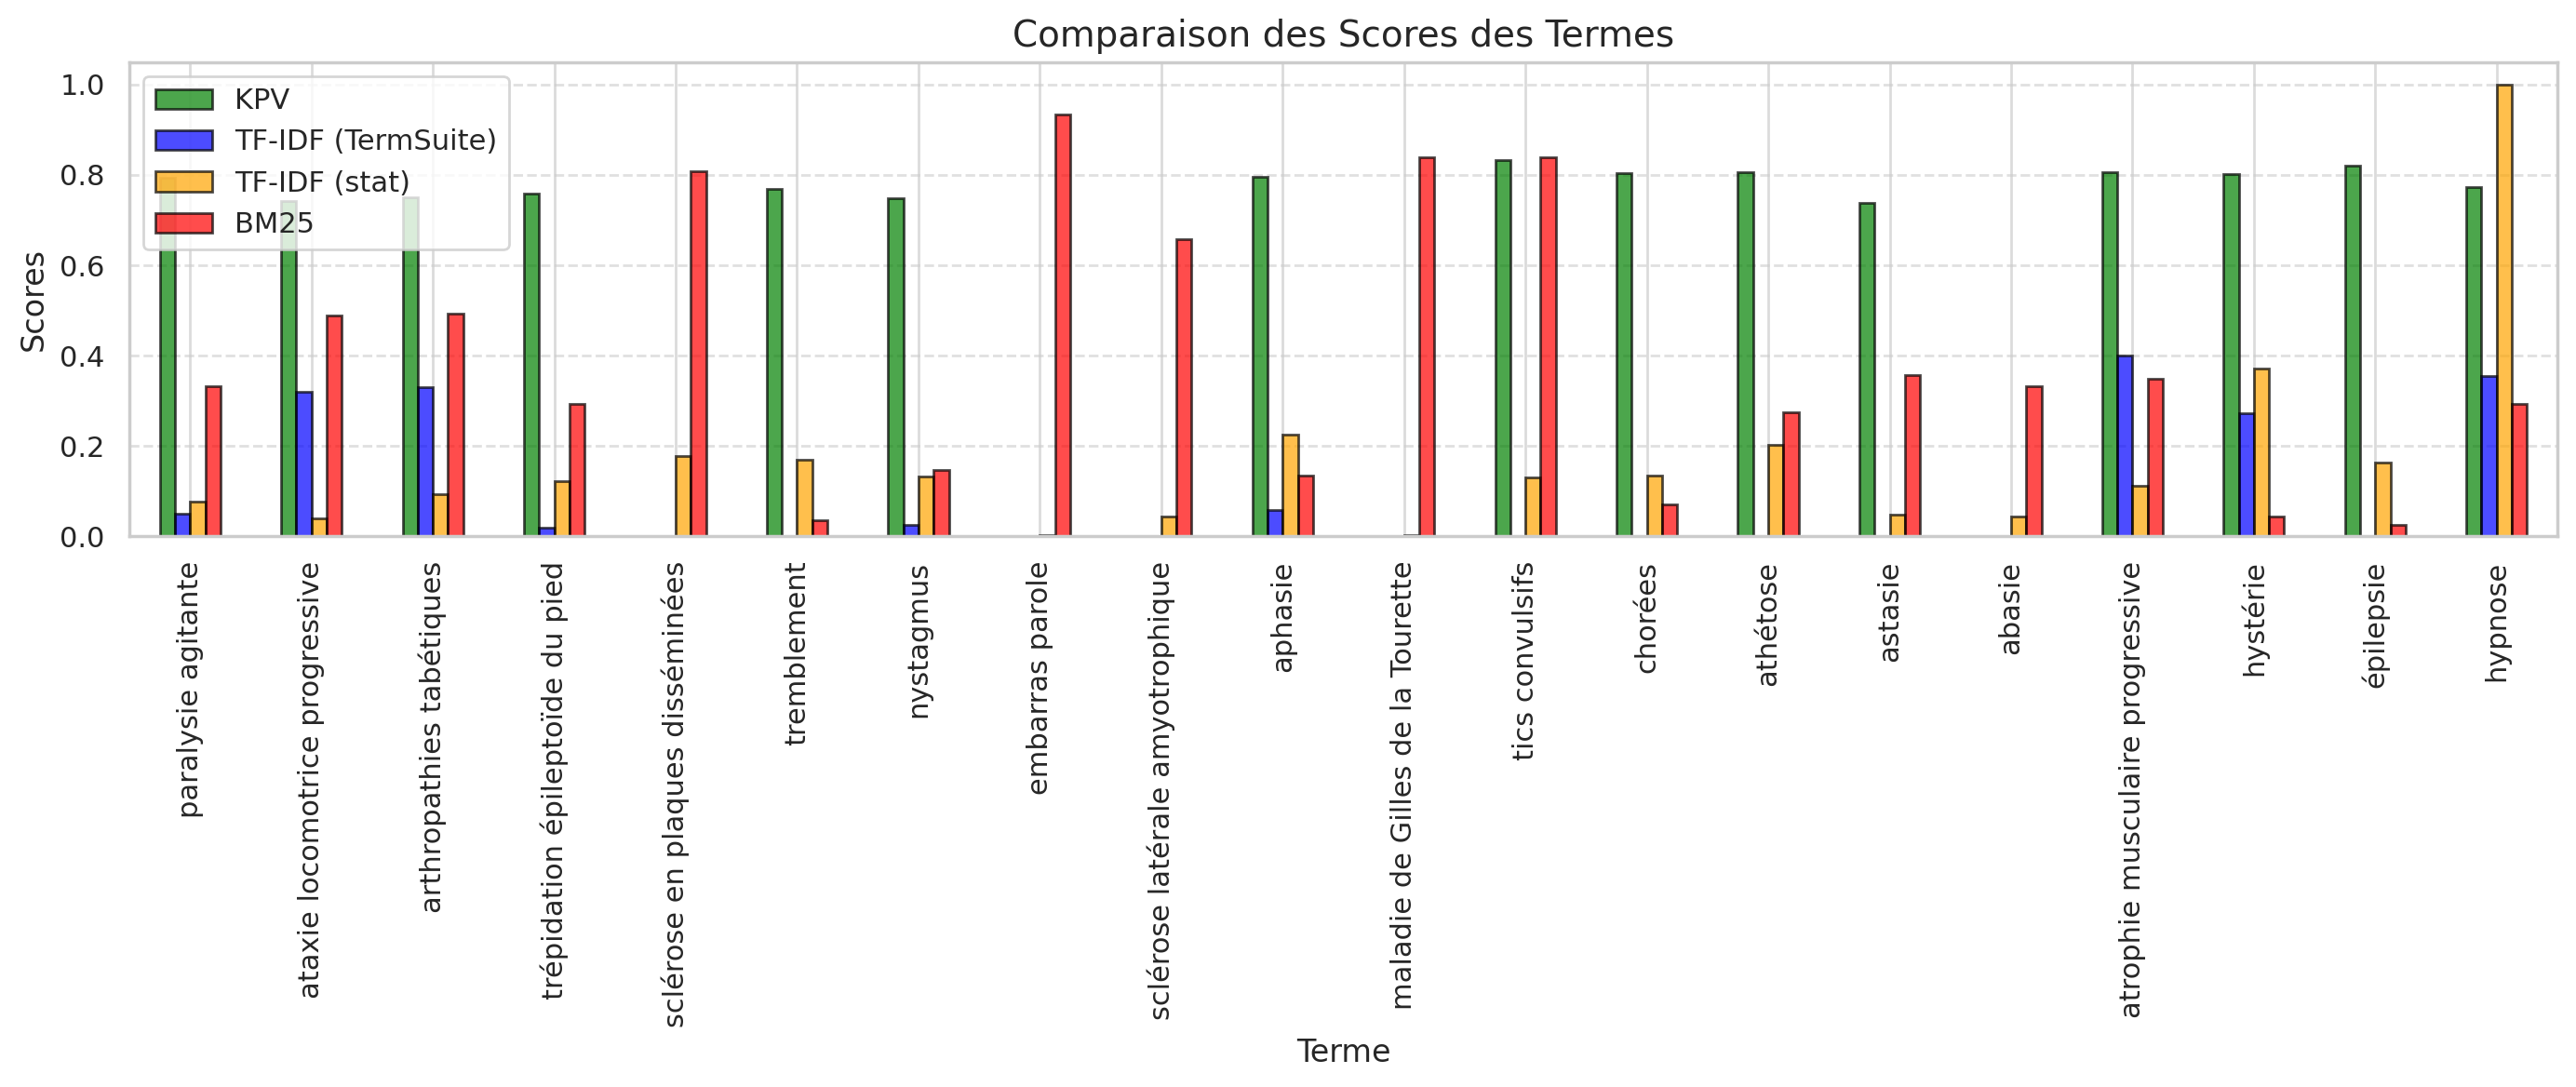
\includegraphics[width=\linewidth]{pic/termes_viz.png}
%	\caption{Visualisation des scores de pertinences pour chaque terme de référence}
%	\label{fig:ling_out_TAL}
%\end{figure}
%\end{frame}

%\begin{frame}{\textit{PatternRank}}
%	Les termes les plus pertinents dans \og{}Autres\fg{} :
%\begin{table}[h]
%	\centering
%	\begin{tabular}{|l|l|c|}
	%		\hline
	%		\textbf{Terme} & \textbf{Synonyme} & \textbf{Score} \\
	%		\hline
	%		\texttt{tics convulsifs} & \bolder{syndrome de Tourette} & \textsc{0.8331} \\
	%		\texttt{état parkinsonien} & \bolder{maladie de Parkinson} & 0.7936 \\
	%%		\texttt{paralytiques agitants} & \bolder{maladie de Parkinson} & 0.7851 \\
	%		\hline
	%	\end{tabular}
%\end{table}
%\end{frame}





%\begin{frame}{Chronologie d'une locution : indice de croissance de l'impact ?}
%\begin{figure}[h] % Use [H] to force the figure to stay in place
%	\begin{itemize}
	%		\item évolution de la fréquence des termes au sein des deux corpus\footnote{\url{https://obtic.huma-num.fr/obvie/charcot/?view=corpus}}
	%		\item convergence entre des termes : fin \textsc{XIX}\ieme{}, début \textsc{XX}\ieme{} s.
	%%		\begin{itemize}
		%%				\item \textit{ppm} : nombre d’occurrences par million de mots 
		%%		\end{itemize}
	%	\end{itemize}
%	\centering
%	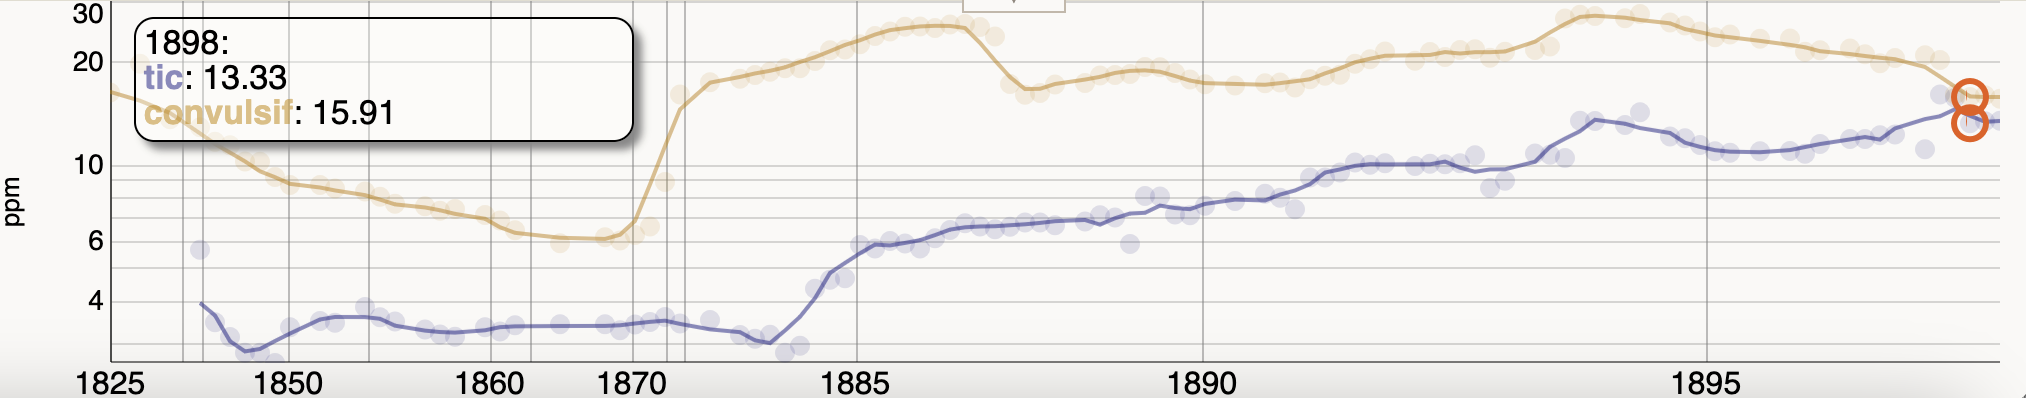
\includegraphics[width=\linewidth]{pic/tics_convulsifs.png}
%	\caption{Chronologie de la fréquence du terme \textit{tic convulsif}.}
%	\label{fig:ling_out_TAL}
%\end{figure}
%
%\begin{figure}[h]
%	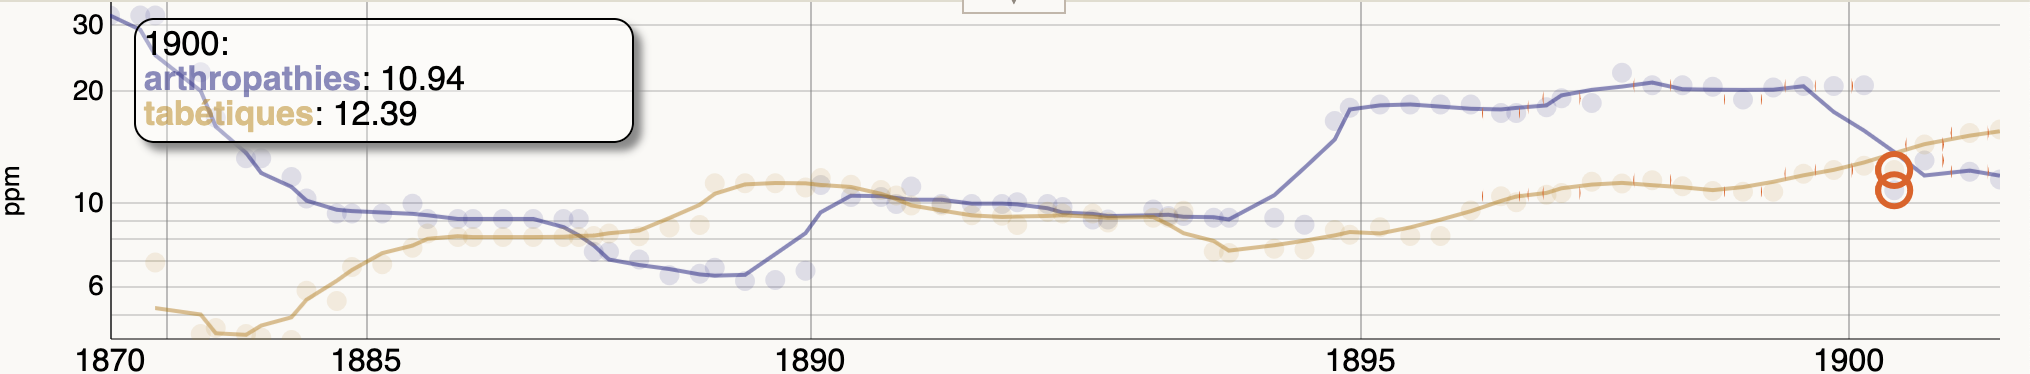
\includegraphics[width=\linewidth]{pic/arthropathies_tabetiques.png}
%\caption{Chronologie de la fréquence du terme \textit{arthropathies tabétiques}.}
%\label{fig:ling_out_TAL}
%\end{figure}
%\end{frame}

%\subsection[Comparaison avec les hypothèses initiales]{Comparaison avec les hypothèses initiales}



%\begin{frame}{Critères de comparaison des approches}
%	\begin{itemize}
%		\item prise en compte des synonymes des termes
%		\begin{itemize}
%			\item ex. \textit{paralysie agitante} $\rightarrow$ \textit{maladie de Parkinson} 
%		\end{itemize}
%					\item recenser le score le plus élevé sur le terme ou sur son synonyme
%					\item les méthodes classiques \textit{vs.} celles de l'état de l'art
%	\end{itemize}
%	
%	\end{frame}
	




%\begin{frame}{\textit{PatternRank}}
%	Les termes les plus pertinents dans \og{}Autres\fg{} :
%\begin{table}[h]
%	\centering
%	\begin{tabular}{|l|l|c|}
%		\hline
%		\textbf{Terme} & \textbf{Synonyme} & \textbf{Score} \\
%		\hline
%		\texttt{tics convulsifs} & \bolder{syndrome de Tourette} & \textsc{0.8331} \\
%		\texttt{état parkinsonien} & \bolder{maladie de Parkinson} & 0.7936 \\
%%		\texttt{paralytiques agitants} & \bolder{maladie de Parkinson} & 0.7851 \\
%		\hline
%	\end{tabular}
%\end{table}
%\end{frame}







\section[Conclusion]{Conclusion et perspectives}
\begin{frame}{Conclusion et perspectives}
	\begin{enumerate}
		\item 	\textit{PatternRank} : la méthode la plus robuste
		\begin{itemize}
			\item capture la sémantique jusqu'aux pentagrammes
			\begin{itemize}
				%				\item quadrigrammes : \textit{sclérose cérébrale tubéreuse hypertrophique} 
				\item \textit{méningite syphilitique hémorragique fibrineuse aiguë}
			\end{itemize}
			\item produit des scores de pertinence plus élevés
			\begin{itemize}
				\item exception : scores BM25 (\textit{SLA}, \textit{embarras parole}) et TF-IDF (\textit{hypnose})
			\end{itemize}
		\end{itemize}
		
		\item 	les termes les plus impactants dans les corpus :
		\begin{itemize}
			\item Charcot : \textit{hystérie}, \textit{astasie-abasie}, \textit{embarras parole}
			\item Autres :  \textit{hypnose}*, \textit{syndrome de Tourette}, \textit{arthropathies tabétiques}
		\end{itemize}

		%		\item Absence des scores pour les termes comme \textit{SEP} et SLA :
		%		\begin{itemize}                                        
			%			\item solution : chercher leurs symptomes ou leurs descriptions :
			%			\begin{itemize}
				%				\item  \textit{amyotrophie spinale progressive}, \textit{secousses nystagmiques}$\dots$
				%			\end{itemize}
			%		\end{itemize}
	\end{enumerate}
	
	\begin{alertblock}{\vspace*{-0.6mm}}
		\centering
		Les résultats sont alignés avec les faits historiques.
	\end{alertblock}
	
	\bigskip
	Recherches futures : tester les \textit{LLM} ou les \textit{LCM} (angl. \textit{Large Concept Models}) ?
\end{frame}

%
%\section[Approche supervisée]{Approche supervisée}
%\input{2_methodo}
%\input{supervise}
%\section[Approche non supervisée]{Approche non supervisée}
%%\begin{frame}{Extraction des phrases-clés}
%\og{}\textcolor{deepblue}{Phrases-clés}\fg{}, angl. \textit{keyphrases}
%\begin{itemize}
%\item séquences de plusieurs mots (ex. \textit{sclérose latérale amyotrophique})
%\item reflètent plus précisément le contexte sémantique du texte \\\small{$\neq$ mots-clés, angl. \textit{keywords} : unigrammes de mot (ex. \textit{sclérose})}
%\end{itemize}
%\bigskip
%%\centering
%%Extraction de \og{}phrases-clés\fg{} (angl. \textit{keyphrases})
%%\\~\\
%%\begin{block}{Extraction de phrases-clés}
%%\justifying
%%Processus de \underline{sélection} automatique d'un petit ensemble de phrases les plus pertinentes à partir d'un texte donné \citep{schopf2022}.
%%\end{block}
%%\begin{block}{Prédiction de phrases-clés}
%%\justifying
%%Processus de \underline{génération} des phrases-clés qui résument parfaitement un document donné \citep{xie2023}.
%\begin{columns}[t,onlytextwidth]
%\column{.45\textwidth}
%\textcolor{violet}{Extraction}
%\justifying
%
%Processus de \underline{sélection} automatique d'un petit ensemble de phrases les plus pertinentes à partir d'un texte donné.
%\vspace{-0.2cm}
%\begin{flushright}
%\small{\citep{schopf2022}}
%\end{flushright} 
%\column{.45\textwidth}
%\textcolor{violet}{Prédiction}
%\justifying
%
%Processus de \underline{génération} des phrases-clés qui résument parfaitement un document donné.
%\vspace{0.3cm}
%\begin{flushright}
%\small{\citep{xie2023}}
%\end{flushright}
%\end{columns}%Extraction de phrases-clés
%%
%%Processus de \underline{sélection} automatique d'un petit ensemble de phrases les plus pertinentes à partir d'un texte donné \citep{schopf2022}.
%%
%%\begin{block}{Prédiction de phrases-clés}
%%\justifying
%%Processus de \underline{génération} des phrases-clés qui résument parfaitement un document donné \citep{xie2023}.
%%\end{block} 
%\end{frame}

\begin{frame}{Extraction des phrases-clés : méthode \texttt{keybert}}
	\begin{enumerate}
		\small
		\item entrée : un document
		\item tokénisation du document en phrases-clés candidates (PCC)
		\item génération des plongements du doc. et des PCC par un modèle de langage
		\item calcul de la similarité cosinus entre le document et les PC
	\end{enumerate}
	\begin{figure}
		\centering
		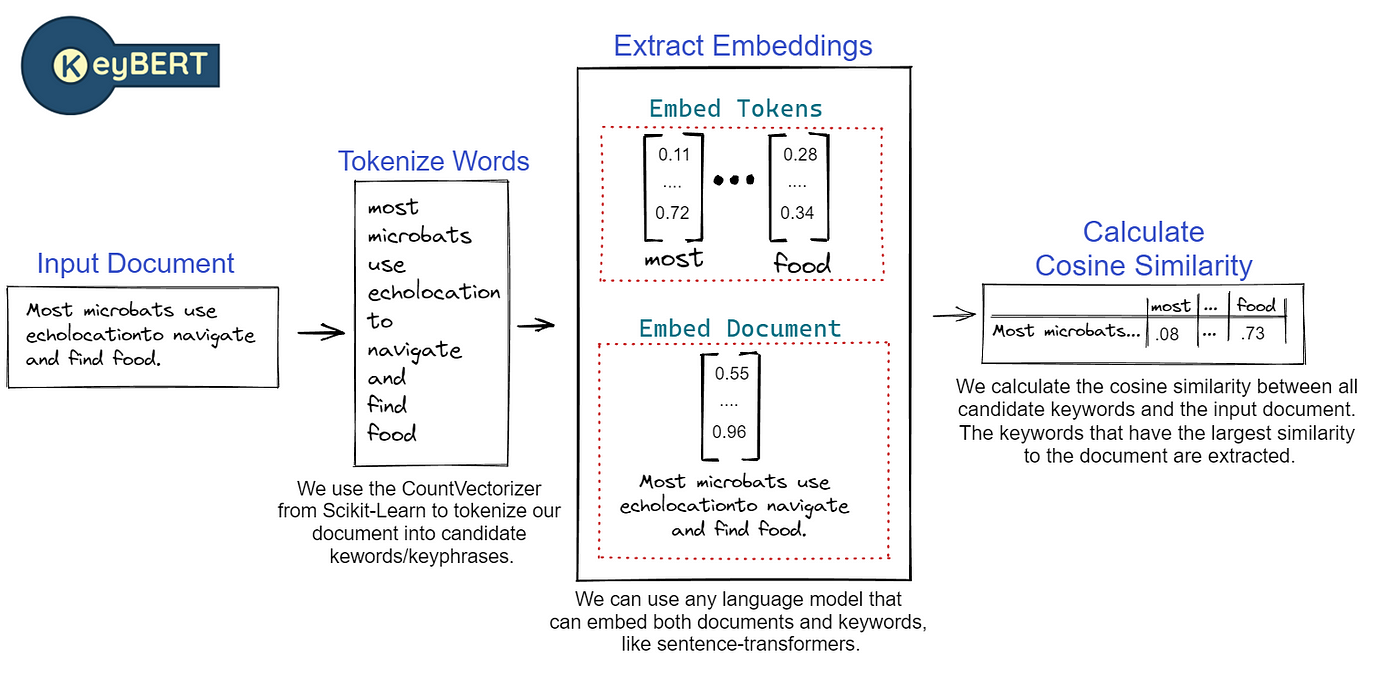
\includegraphics[width=80mm,scale=0.5]{pic/keybert.png}
		\caption{\textit{Pipeline} de la librairie \texttt{keybert} \citep{grootendorst2020keybert}.}
		\label{fig:enter-label}
	\end{figure}
\end{frame}

\begin{frame}{Extraction des phrases-clés : méthode \textit{PatternRank}\\
		\quad \quad \quad\ \quad \quad \quad \quad \quad \quad \quad \ \ \ \ \ \small{Librairie \texttt{keyphrase-vectorizers}}}
	%\begin{itemize}
	%\item extraction des phrases-clés non-supervisée
	%\item exploite des modèles de langues pré-entraînés + parties du discours
	%\end{itemize}
	\begin{enumerate}
		\small
		\item entrée : un seul document texte tokenisé
		\item étiquetage des tokens avec les balises du partie du discours (POS)
		\item sélection des tokens selon le motif POS $\rightarrow$ phrases-clés candidates (PCC)
		\item génération des plongements du doc. et des PCC par un modèle de langue
		\item calcul des similarités cosinus entre ces deux types de plongements +  \\classement des PCC par ordre décroissant
		\item extraction des \textit{N} PC les plus représentatives
	\end{enumerate}
	\begin{figure}
		\centering
		\includegraphics[width=110mm,scale=0.5]{pic/patternrank\_workflow.png}
		\caption{\textit{Workflow} de la méthode \textit{PatternRank} \citep{schopf2022}.}
		\label{fig:enter-label}
	\end{figure}
	\notecite{schopf2022}
\end{frame}



%\section[Conclusion]{Conclusion et recherches futures}
%\begin{frame}{Conclusion et perspectives}
	\begin{enumerate}
		\item 	\textit{PatternRank} : la méthode la plus robuste
		\begin{itemize}
			\item capture la sémantique jusqu'aux pentagrammes
			\begin{itemize}
				%				\item quadrigrammes : \textit{sclérose cérébrale tubéreuse hypertrophique} 
				\item \textit{méningite syphilitique hémorragique fibrineuse aiguë}
			\end{itemize}
			\item produit des scores de pertinence plus élevés
			\begin{itemize}
				\item exception : scores BM25 (\textit{SLA}, \textit{embarras parole}) et TF-IDF (\textit{hypnose})
			\end{itemize}
		\end{itemize}
		
		\item 	les termes les plus impactants dans les corpus :
		\begin{itemize}
			\item Charcot : \textit{hystérie}, \textit{astasie-abasie}, \textit{embarras parole}
			\item Autres :  \textit{hypnose}*, \textit{syndrome de Tourette}, \textit{arthropathies tabétiques}
		\end{itemize}

		%		\item Absence des scores pour les termes comme \textit{SEP} et SLA :
		%		\begin{itemize}                                        
			%			\item solution : chercher leurs symptomes ou leurs descriptions :
			%			\begin{itemize}
				%				\item  \textit{amyotrophie spinale progressive}, \textit{secousses nystagmiques}$\dots$
				%			\end{itemize}
			%		\end{itemize}
	\end{enumerate}
	
	\begin{alertblock}{\vspace*{-0.6mm}}
		\centering
		Les résultats sont alignés avec les faits historiques.
	\end{alertblock}
	
	\bigskip
	Recherches futures : tester les \textit{LLM} ou les \textit{LCM} (angl. \textit{Large Concept Models}) ?
\end{frame}
%\section[État de l'art]{État de l'art}
%\input{sota}
%\section[\textit{PatternRank}]{\textit{PatternRank}}
%\input{patternrank}



% \appendix

\begin{frame}[allowframebreaks]{Références}
\printbibliography

\end{frame}

\end{document}